\documentclass[reprint, superscriptaddress, floatfix]{revtex4-1}
\usepackage{amsmath}
\usepackage{mathtools}
\usepackage{upgreek}
\usepackage[table,usenames,dvipsnames]{xcolor}
\usepackage{tikz}
\usetikzlibrary{calc}
\usepackage{hyperref}
\usepackage{setspace}

\hypersetup{
  colorlinks,
  linkcolor={red!30!black},
  citecolor={green!20!black},
  urlcolor={blue!80!black}
}


\definecolor{DarkBlue}{RGB}{0,0,64}
\definecolor{DarkBrown}{RGB}{64,20,10}
\definecolor{DarkGreen}{RGB}{0,64,0}
\definecolor{DarkPurple}{RGB}{64,0,42}
\definecolor{LightGray}{gray}{0.85}
% annotation macros
\newcommand{\repl}[2]{{\color{gray} [#1] }{\color{blue} #2}}
\newcommand{\add}[1]{{\color{blue} #1}}
\newcommand{\del}[1]{{\color{gray} [#1]}}
\newcommand{\note}[1]{{\color{DarkGreen}\footnotesize \textsc{Note.} #1}}
\newcommand{\answer}[1]{{\color{DarkBlue}\footnotesize \textsc{Answer.} #1}}
\newcommand{\summary}[1]{{\color{DarkPurple}\footnotesize \textsc{Summary.} #1}}


\newcommand{\Err}{E}
\newcommand{\ii}{\mathrm{i}}



\begin{document}



\title{Optimal updating factor in adaptive flat-distribution-sampling simulations}

\author{Cheng Zhang}
\author{Justin A. Drake}
\affiliation{
Sealy Center for Structural Biology and Molecular Biophysics,
The University of Texas Medical Branch,
Galveston, Texas 77555-0304, USA}
\author{Jianpeng Ma}
\affiliation{
Department of Biochemistry and Molecular Biology,
Baylor College of Medicine, Houston, Texas 77030, USA}
\affiliation{
Department of Bioengineering,
Rice University, Houston, Texas 77005, USA}
\author{B. Montgomery Pettitt}
\email{bmpettitt@utmb.edu}
\affiliation{
Sealy Center for Structural Biology and Molecular Biophysics,
The University of Texas Medical Branch,
Galveston, Texas 77555-0304, USA}



\begin{abstract}
  We present a method of computing the optimal schedule
  of the updating magnitude
  for a class of free energy calculation methods including
  the Wang-Landau (WL) algorithm and metadynamics.
  %
  These methods rely on adaptive construction of
  a bias potential that offsets
  the potential of mean force by histogram-based adaptive updates.
  %
  The updating magnitude should decrease over time
  to reduce the noise in the bias potential,
  and one may speed up the convergence by choosing an optimal schedule
  of the updating magnitude.
  %
  %Here, we will show that the optimal schedule
  %can be derived
  %from a mechanical analogy, in which
  %the schedule corresponds to
  %the velocity of a free particle with a position-dependent mass
  %and the final error serves as the action.
  %%
  %Therefore, the optimal schedule follows from
  %the equation of motion of the particle.
  %
  We will show that
  the optimal schedule depends on the updating scheme (WL or metadynamics),
  and the initial updating magnitude is ideally half of
  the previous equilibrium value.
  %
  Further,
  the WL updating scheme
  belongs to a class of bandpass updating schemes
  that are optimal for asymptotic convergence,
  and the optimal schedule of these schemes
  is the inverse number of sampling steps with a proper shift,
  as given by the $1/t$ prescription.
  %
\end{abstract}

\maketitle



\section{Introduction}



Free energy calculation\cite{frenkel, newman} is a central theme
in computational physics and chemistry
that can provide insight into an array of phenomena not easily studied
with traditional experiments.
%
Given a system,
often the task is to compute
a distribution, $p^*(z)$,
along a collective variable, $z$, by sampling via either Monte Carlo\cite{
  frenkel, newman, landau_binder} (MC)
or molecular dynamics\cite{frenkel, karplus2002} (MD) simulations.
%
The dimensionless free energy, or potential of mean force (PMF),
along the collective variable, $z$,
is $-\ln p^*(z)$.
%
However, accurately estimating the PMF is often difficult
when the collective variable is energetically restricted to local regions
of the complex, multi-modal free energy surface.
%
Thus,
to overcome these energetic barriers and
to capture the global shape of the free energy surface
an effective strategy is to introduce a bias potential that
cancels the PMF.
%
Ideally, then, sampling yields a flat distribution
along $z$\cite{mezei1987, berg1992, *lee1993,
wang2001, *wang2001pre,
huber1994,
*laio2002, *laio2008, *barducci2011, *sutto2012}.
%
The flat-distribution sampling can be used to accelerate
sampling of slow transitions that otherwise would not readily
be observed with traditional simulations.
%
%A better solution is to artificially flatten
%the target distribution along $z$\cite{mezei1987, berg1992, *lee1993,
%wang2001, *wang2001pre,
%huber1994,
%*laio2002, *laio2008, *barducci2011, *sutto2012}.
%%
%This alleviates the above problem of local trapping
%by forcing the system to travel more
%deliberately along $z$,
%which often represents
%a direction of slow motion.
%%
%To achieve a flat distribution, however,
%the method must be able to construct a
%bias potential that cancels the PMF.



Many efficient flat-distribution-sampling (FDS) techniques
based on adaptive construction of the bias potential
have been introduced,
including the Wang-Landau (WL) algorithm\cite{
  wang2001, *wang2001pre}
and metadynamics\cite{huber1994,
*laio2002, *laio2008, *barducci2011, *sutto2012},
more commonly used for MC and MD simulations, respectively\cite{junghans2014}.
%
%flat-distribution-sampling (FDS) techniques
%that build the bias potential adaptively or on the fly.
%
These techniques regularly update the bias potential
to discourage future visits to previously sampled configurations
by incrementally elevating the bias potential,
%and they are closely-related\cite{junghans2014, micheletti2004}.
%
%The bias potential is associated with discrete values of $z$.
%
A key difference lies
in the updating window function,
which specifies
a neighborhood around the current value of $z$ on the free energy surface
where the updating should occur
as well as the relative updating magnitude.
%
Usually, the window function
takes the form of a discrete
$\delta$-function (a boxcar function one histogram bin wide)
in WL,
or that of a Gaussian
in metadynamics.
%
Although the assignment of the window functions to the two methods
is not absolute\cite{micheletti2004, kim2006, *kim2007, junghans2014},
below we will use the terms WL and metadynamics
to represent FDS simulations using the
$\delta$- and Gaussian window functions, respectively.
%
%is that in the WL case,
%each updating step is limited to the bin
%containing the current $z$,
%while metadynamics adopts an extended
%Gaussian window
%covering several neighboring bins.
%%
%The latter is more often used in MD simulations
%as it guarantees a smooth profile
%of the bias potential
%suitable for numerical differentiation
%in deriving the bias force.
%
In both cases,
regular updates to the bias potential
%in both cases, the bias potential
%is updated frequently (usually every few MC or MD steps),
%and the fluctuation
disrupts the underlying equilibrium
sampling\cite{zhou2005, morozov2007, zhou2008},
and for convergence of the estimated PMF
one  has to gradually decrease
the updating magnitude of the bias.



The schedule of reducing
the updating magnitude,
therefore, critically affects
the precision of the final bias potential,
and hence that of the PMF\cite{
belardinelli2007, *belardinelli2007jcp, *belardinelli2008, *belardinelli2016,
liang2007,
morozov2007, zhou2008,
komura2012, *caparica2012, *caparica2014,
barducci2008, dickson2011, dama2014}.
%
For the WL algorithm, the optimal updating schedule
is a function of the
inverse time\cite{
belardinelli2007, *belardinelli2007jcp, *belardinelli2008, *belardinelli2016,
liang2007,
morozov2007, zhou2008}
or
the inverse number of simulation steps.
\note{
  About the origin of the inverse-time formula.
  Besides the Belardinelli paper,
  we can also find it in Eq. (6) of reference \cite{liang2007},
  if I am not too mistaken.
  But I find the paper is a bit hard to read.
  There, however, the formula is $t_0/t$ instead of $1/t$.
}
%
%The optimal schedule for metadynamics,
%however, is less studied.


In this study,
we present a method of computing
the optimal schedule
for an adaptive FDS method
with a general window function,
including the $\delta$- and Gaussian one
used in the WL algorithm and metadynamics.
%
Our method maps the optimization problem to a mechanical one,
in which the schedule plays the role of the velocity of
a free particle with a position-dependent mass,
and the final error becomes the action.
%
In this way, the optimal schedule
can be deduced from the equation of motion
of the particle that minimizes the action.
%
As the mass is defined from the updating window function,
the resulting optimal schedule
is different in the WL and metadynamics cases.
%
While the optimal schedule in the WL case
is given by the known inverse-time formula,
the optimal schedule for metadynamics is more complex
and sensitive to the simulation length
and the width of the Gaussian window.
%
In either case, however,
the initial updating magnitude
can be optimally set to
half of the previous equilibrium value,
which amounts to a shift of the origin of time in the WL case.
%
Further, we can generalize
the WL updating scheme
to a class of bandpass updating schemes
that are optimal for long simulations,
and the above origin-shifted inverse-time schedule
turns out to be optimal for these schemes.
%
%For finite-length simulations, however,
%metadynamics may deliver better performance.
%
These results may help to better
plan and optimize FDS simulations.



The article is organized as follows.
%
We present the analytical results in Sec. \ref{sec:theory},
numerically verify some aspects
in Sec. \ref{sec:results},
and conclude the article
in Sec. \ref{sec:conclusion}.




\section{\label{sec:theory}
Theory}



We develop the theory
in the following order.
%
In Sec. \ref{sec:background},
we first review the basics of FDS
and some known aspects of the optimal schedule.
%
Then, in Sec. \ref{sec:single-bin},
we illustrate the method of
computing the optimal schedule
in the simple case of the
single-bin updating scheme
used by the WL algorithm,
by proving the optimality
of the known inverse-time formula.
%
The above two introductory sections help fix our notations,
and an expert reader can readily skip them.
%
Next, we extend the method to the general case
of a multiple-bin updating scheme
that encompasses metadynamics
in Secs. \ref{sec:multiple-bin}
to \ref{sec:band-matrix}.
%
Finally, we compare different updating schemes
and show that the single-bin scheme
and a class of generalized bandpass schemes
are optimal for convergence
in the long time or extensive sampling limit
in Sec. \ref{sec:cmpschemes}.



\subsection{\label{sec:background}
Background}



\subsubsection{\label{sec:FDS}
Flat-distribution sampling}



Consider the problem of computing
the distribution, $p^*_i$,
along a discrete quantity, $i$,
for a given system.
%
%The discreteness of $i$ is natural
%in discrete models.
%
For example, $i$ can be the energy, $E$,
in a lattice spin model or the temperature index
in a simulated tempering simulation\cite{
marinari1992, *lyubartsev1992}.
%
For a continuous quantity, $z$,
which is often the case in a (classical) molecular system,
we can discretize $z$
such that the integer $i$ represents
the index of a small interval, or a bin,
$(z, z + \Delta z)$.
%
The distribution is normalized as
$\sum_{i = 1}^n p^*_i = 1$.



%For a large system at temperatures of interest,
%the distribution, $p^*_i$, often tends to
%be localized,
%%
%and to explore the global shape
%of the PMF, $-\ln p^*_i$,
%it is often advantageous to perform
%biased sampling that targets
%a wider and smoother distribution, $p_i$.
%%
%%Here, we refer to simulations that target
%%a flat or nearly flat distribution
%%as entropic or multicanonical sampling.
%
%To do so, we introduce a bias potential, $V_i$,
If the distribution, $p^*_i$, is multimodal,
it is often advantageous to perform
biased sampling that targets
a smoother distribution, $p_i$,
by introducing a bias potential, $V_i$,
such that the biased equilibrium distribution is
%
\begin{equation}
  \pi_i
  %=
  %C_i \, p^*_i \, e^{-V_i}
  =
  \frac{                p^*_i \, e^{-V_i} }
       { \sum_{j = 1}^n p^*_j \, e^{-V_j} }
  \propto
  p^*_i \, e^{-V_i}
  .
  \label{eq:pi_p_V}
\end{equation}
%
%where the proportionality constant, $C_i$,
%is found from the normalization condition,
%$\sum_{i = 1}^n \pi_i = 1$,
%in the second step.
%
%In particular,
%to make $\pi_i$ flat,
%the bias potential $V_i$
%must coincide with $\ln p^*_i$,
%up to an additive constant.
%%
%In practice, $V_i$ may be non-optimal or contain error,
%and thus $\pi_i$ need not
%coincide with the intended distribution $p_i$.

We will broadly call a biased simulation
targeting a flat (i.e. $p_i \equiv 1/n$)
or nearly flat\cite{
dayal2004, *trebst2004, *zhang2007, barducci2008, singh2011}
$p_i$
a flat-distribution-sampling (FDS) simulation.
%
For the biased distribution, $\pi_i$,
to converge to $p_i$,
the bias potential must satisfy
%
\begin{equation}
  V_i \to \ln p^*_i - \ln p_i + \mathrm{const.}
  .
  \label{eq:Vi_target}
\end{equation}
%
%according to Eq. \eqref{eq:pi_p_V}.
%which allows us to deduce the PMF, $-\ln p^*_i$,
%directly from the bias potential.
%
In practice,
the bias potential is adjusted to make the
observed distribution, or the normalized histogram,
match the intended one,
and once this is done,
the PMF, $-\ln p^*_i$, can be naturally
deduced from the bias potential. % $V_i$.
%
%This relation thus sets a practical aim for the convergence of FDS
%methods---the bias potential must be adjusted to make the
%observed distribution, or the normalized histogram,
%match the intended one.
%%
%Once this aim is achieved,
%the PMF, $-\ln p^*_i$, can be naturally
%deduced from the bias potential. % $V_i$.
\note{
  For example, in the context of simulated tempering (Zhang and Ma, 2007),
  $p^*_i$ is replaced by $\ln Z_i$,
  $p_i$ is the weight $\zeta_i$,
  and the bias potential, $V_i$, is $\ln (\tilde Z_i / \zeta_i)$.
  Upon convergence, we have $\ln \tilde Z_i \to \ln Z_i$
  up to a constant shift.
}



Roughly speaking, there are two types of FDS methods.
%
The first type,
referred to as the equilibrium FDS, % (E-FDS) methods hereinafter,
uses a fixed bias potential, $V_i$,
(estimated a priori)
during simulation.
%
Examples include the original
entropic or multicanonical sampling\cite{
berg1992, *lee1993}
and simulated tempering\cite{
marinari1992, *lyubartsev1992}.
%with $i$ being the index of energy
%and that of temperature, respectively.
%
The estimated bias potentials at bin $i$, $V_i$,
are often improved
with the normalized histogram of the sampling, $H_i$, accumulated
during simulation.
%
Using $H_i$ as an estimate of $\pi_i$ in
Eq. \eqref{eq:pi_p_V}
allows us to correct $V_i$ as
%
\begin{equation}
  V^\mathrm{corr}_i
  =
  V_i
  +
  \ln \frac{ H_i }
           { p_i }.
  \label{eq:vcorr_equil}
\end{equation}
%
\note{This follows from
  $$
  \begin{aligned}
    H_i \approx \pi_i
    &\propto p^*_i \, e^{-V_i},
    \\
    p_i
    &\propto p^*_i \, e^{-V^\mathrm{corr}_i}.
  \end{aligned}
  $$
}
%However, for an unknown system,
%it is often difficult
%to guess a sufficiently accurate
%$V_i$ with which to start.
%%
%Thus,
%it can take many iterative rounds of simulations
%to achieve the desired flat distribution.
%%
%%Another difficulty of this approach is that
%The effectiveness of this approach
%depends on the precision of the histogram, $H_i$,
%which in turn depends on the simulation length
%that must be decided in advance.
However, this formula often requires a long
simulation period to accumulate a precise histogram, $H_i$,
and thus it disallows
continuous improvement of the bias potential
(hence that of the PMF)
as simulation lengthens.

The second type of methods,
including the WL algorithm and metadynamics,
address the above shortcomings
by continuously and incrementally updating the bias potential.
%For this reason, the second type of methods,
%referred to as the adaptive FDS methods,
%were invented.
%
These methods, refered to as the adaptive FDS methods,
will be discussed below.
%%
%%These methods incrementally update the bias potential
%%and can approximately sample the target distribution.
%%
%However,
%the on-the-fly updates break the microscopic reversibility
%of the underlying sampling mechanism.
%Further, failure to properly reduce the magnitude of
%the histogram-based increments
%would lead to roughness or errors in the final estimate of the PMF.
%%
%%Thus, for a conservative practitioner,
%%the E-FDS methods appear more appealing
%%once a sufficiently accurate bias potential is available.
%%
%To minimize this effect,
%many adaptive methods adopt a schedule to
%reduce the updating magnitude
%over the course of simulation\cite{
%marsili2006,
%belardinelli2007, *belardinelli2007jcp, *belardinelli2008, *belardinelli2016,
%liang2007,
%barducci2008}.
%%
%%Thus, in late stages of a long simulation,
%%the updating becomes negligible and
%%the adaptive simulation tends to
%%the corresponding equilibrium one.
%%
%%if the bias potential were converged to the exact value,
%%this adaptive FDS tends to the ideal equilibrium counterpart,
%%particular equilibrium simulation can be thought as
%%the optimal asymptotic limit of the adaptive counterpart,
%%
%For example, one can show that
%if the magnitude is controlled by
%the optimal inverse-time prescription\cite{
%belardinelli2007, *belardinelli2007jcp, *belardinelli2008, *belardinelli2016,
%liang2007,
%morozov2007, zhou2008,
%komura2012, *caparica2012, *caparica2014},
%the WL algorithm is equivalent to the ideal equilibrium counterpart
%in improving the precision of the bias potential,
%thus allowing for maximum efficiency
%(cf. Appendix \ref{sec:equilerr}).
%%the bias potential in the WL algorithm
%%will evolve similar to Eq. \eqref{eq:vcorr_equil}
%%with the precision of the histogram as simulation lengthens.


\subsubsection{Updating schemes}



%We will mainly focus on the adaptive methods below.
%
In the WL algorithm\cite{wang2001, *wang2001pre},
the bias potential, $V_i(t)$, is updated
at each sampling step $t$ as
%
\begin{equation}
  V_i(t+1)
  =
  V_i(t)
  +
  \delta_{i, \, i(t)}
  \frac{ \alpha(t) } { p_{i(t)} }
  ,
\label{eq:wl_update}
\end{equation}
%
where $i(t)$ is the bin at step $t$,
$\delta_{i, \, i(t)}$ is the Kronecker delta function,
which is $1$ when $i = i(t)$ or $0$ otherwise,
and $\alpha(t)$ is the updating magnitude.
%
We refer to this scheme as the \emph{single-bin scheme},
for it applies only to the bias potential
at the current bin, $i(t)$.
%
In a more general \emph{multiple-bin scheme}, however,
several neighboring bins are updated:
%
\begin{equation}
  V_i(t+1)
  =
  V_i(t)
  +
  w_{i, \, i(t)}
  \frac{ \alpha(t) }
       { p_{i(t)} },
  \label{eq:mbin_update}
\end{equation}
%
where the elements, $w_{ij}$'s, are a set of coefficients satisfying
the restrictions to be discussed
in Sec. \ref{sec:updating-matrix}.
%
The Gaussian updating scheme
used in metadynamics
is a multiple-bin scheme.



One can show that with a constant magnitude,
$\alpha(t) = \alpha > 0$,
the distribution collected from
an adaptive FDS simulation
is identical to $p_i$ in the long time or asymptotic limit.
%
However, as the above updates
change $V_i(t)$ continuously,
the equilibrium distribution,
Eq. \eqref{eq:pi_p_V}, no longer holds
at all times,
and the error in $V_i(t)$
depends on the updating magnitude\cite{
  belardinelli2007, *belardinelli2007jcp, *belardinelli2008, *belardinelli2016,
  zhou2005, morozov2007, zhou2008,
  laio2005, bussi2006, poulain2006, liang2007,
  crespo2010, *atchade2011, *fort2015}.
%%
%The source of the deviation is two-fold.
%%
%First, since $V_i(t)$ is updated continuously,
%there is a random noise that is proportional
%to $\sqrt \alpha$.
%%
%Second, there is a systematic error
%that comes from the updating dynamics itself,
%as it breaks the Markovian nature
%that underlies Eq. \eqref{eq:pi_p_v}.
%%
%
Thus, one has to reduce the magnitude, $\alpha$, over time
to improve the estimate of the distribution,
$p^*_i$. %via Eq. \eqref{eq:v_def}.





\subsubsection{Updating magnitude and the inverse-time formula}



In the original WL papers\cite{
wang2001, *wang2001pre},
the updating magnitude, $\alpha$,
(or $\ln f$ therein)
is controlled in stages.
%
In each stage, $\alpha$
is kept constant,
and the histogram along $i$
is collected and monitored.
%
Once the histogram is sufficiently flat,
we switch to a new stage
with $\alpha$ reduced by a factor of $1/2$\cite{
wang2001, *wang2001pre}.
%
While this scheme works well for early stages,
%
it tends to reduce $\alpha$
too quickly in late stages, making the asymptotic error
saturate\cite{
belardinelli2007, *belardinelli2007jcp, *belardinelli2008, *belardinelli2016}.


%For the single-bin scheme
%used in WL algorithm,
Later,
it was found that
a better way
of controlling the schedule, $\alpha(t)$,
in late stages
is to follow the formula
%
\begin{equation}
  \alpha(t) = \frac{1}{t},
  \label{eq:alpha_invt}
\end{equation}
%
where $t$,
referred to as the ``time'' below,
is the number of steps
from the beginning of the simulation.
%
This simple yet effective formula has attracted
several studies\cite{
belardinelli2007, *belardinelli2007jcp, *belardinelli2008, *belardinelli2016,
morozov2007, zhou2008,
komura2012, *caparica2012, *caparica2014}.
%
An interesting explanation\cite{
  marsili2006, barducci2008}
comes from the interpretation of
the bias potential %under the WL updating scheme, Eq. \eqref{eq:wl_update},
as a runtime average computed from all data points collected so far,
so that the addition of a new data point only
affects the average by its due weight, $1/t$,
which is the inverse of the current sample size, $t$
(cf. Appendix \ref{sec:equilerr}).
%
Here we will re-derive this formula
and suggest a slight modification
whereby the origin of $t$ is shifted
according to the initial error.
%
Interestingly, we may reach the same result
from optimally planning the simulation lengths in the stages
and the reduction factor, as shown in Appendix \ref{sec:wltoinvt}.


%As Eq. \eqref{eq:alpha_invt} was being developed for the WL algorithm,
%several similar ways of
%reducing the updating magnitude
%were developed for umbrella sampling and metadynamics,
%particularly, the self-healing umbrella sampling
%and well-tempered metadynamics\cite{
%  marsili2006, barducci2008, dickson2011, dama2014}.
%%
Our aim here is to find the optimal schedule, $\alpha(t)$,
for a general updating scheme.




\subsection{\label{sec:single-bin}
Single-bin updating scheme}



In this section,
we will derive the optimal $\alpha(t)$
for the single-bin scheme,
Eq. \eqref{eq:wl_update}.
%
To do so,
we will first express the error of
the bias potential, $V_i(t)$,
as a functional of $\alpha(t)$,
and then minimize it by variation.



\subsubsection{Error}



First, we need to define the error in the bias potential.
%
This is done by deducting two contributions from the bias potential.
%
The first contribution comes from the target value,
Eq. \eqref{eq:Vi_target}.
%
For this purpose,
we introduce a shifted bias potential
%
\begin{equation}
  v_i(t)
  \equiv
  V_i(t)
  -
  \ln \frac { p^*_i }
            { p_i }
  ,
  \label{eq:v_def}
\end{equation}
%
which should tend to a constant of $i$
upon convergence.
Note that the updates to $v_i$'s are
equivalent to the updates to $V_i$'s,
since the shift
remains a constant during the course of simulation,
%%
%In terms of $v_i$'s, Eq. \eqref{eq:pi_p_V}
%becomes
%%
%\begin{equation}
%  \pi_i
%  =
%  \frac{                p_i \, e^{-v_i} }
%       { \sum_{j = 1}^n p_j \, e^{-v_j} }
%  \propto
%  p_i \, e^{-v_i}.
%  \label{eq:pi_p_v}
%\end{equation}
%%
%According to Eq. \eqref{eq:pi_p_V},


Second, the bias potential following Eq. \eqref{eq:wl_update}
generally grows over time.
%
Since a uniform increase of $V_i(t)$, or, equivalently, that of $v_i(t)$,
does not affect the
resulting distribution, $\pi_i(t)$,
%
the real deviation is more readily defined
from the difference between $v_i(t)$ and a baseline value, $\bar v(t)$,
that represents the average growth\cite{
dama2014},
%
\begin{equation}
  x_i(t) \equiv v_i(t) - \bar v(t)
  %=
  %v_i - \sum_{j = 1}^n \rho_j \, v_j
  ,
\label{eq:x_def}
\end{equation}
%
where
%
\begin{equation}
  \bar v(t)
  = \sum_{i = 1}^n \rho_i \, v_i(t)
  ,
\label{eq:vbar_def}
\end{equation}
for some distribution,
$\pmb \rho = (\rho_1, \dots, \rho_n)$
(with $\rho_i \ge 0$ and $\sum_{i = 1}^n \rho_i = 1$).
%
In this way,
the variable, $x_i(t)$,
represents the actual deviation of the bias potential, $V_i(t)$,
and the total error is given by
%
\begin{equation}
  \Err(t)
  =
  \sum_{i = 1}^n \rho_i \, \left\langle x_i^2(t) \right\rangle
  .
\label{eq:error_sum}
\end{equation}




Note that the distribution, $\pmb \rho$,
introduced above to define the error
is independent of
the target distribution,
$\mathbf p = (p_1, \dots, p_n)$.
%
For example,
in well-tempered metadynamics,
$\pmb\rho$ is a flat distribution,
while $\mathbf p$ is an attenuated version of
$\mathbf p^*$\cite{
  barducci2008, dama2014} ($\ln p_i = \ln {p^*_i}/(1+\Delta) + \mathrm{const.}$ for some positive $\Delta$).
%
From Eqs. \eqref{eq:x_def} and \eqref{eq:vbar_def},
we have
%
\begin{equation}
  \sum_{i = 1}^n \rho_i \, x_i(t) = 0
  .
\label{eq:rhox_sum}
\end{equation}
%


\subsubsection{Differential equation}



To proceed, we will
approximate the finite difference Eq. \eqref{eq:wl_update}
by a differential equation
%
\begin{equation}
  \dot V_i(t)
  \equiv
  \frac{ dV_i(t) } { dt }
  =
  \alpha(t) \, \frac{ h_i(t) } { p_i },
  \label{eq:vt_diffeq}
\end{equation}
%
with
%
$
h_i(t) = \delta_{i, i(t)}
$
%\begin{equation}
%  h_i(t) = \delta_{i, i(t)}
%  ,
%  \label{eq:h_def}
%\end{equation}
%
being the instantaneous histogram,
which is equal to $1.0$
for the bin $i(t)$ at time $t$
or zero otherwise.
%
The shifted bias potential, $v_i(t)$,
follows the same differential equation
as the shift is a constant.


Next, we split $h_i(t)$ into a deterministic averaged part
and a stochastic part, $\zeta_i(t)$,
%
\begin{equation}
  h_i(t) = \langle h_i(t) \rangle + \zeta_i(t).
  \label{eq:h_split}
\end{equation}
%
The deterministic part can be related
to an ``ensemble average'',
where the ensemble consists of many similar simulation copies
sharing the same schedule $\alpha(t)$
and the same bias potential at time $t$.
%
The initial states and the stochastic forces
during the process may differ, however.



For sufficiently small $\alpha(t)$,
the bias potential remains roughly the same for a short period.
%
Then,
the sampling process is approximately Markovian, % of a finite order,
and we may assume Eq. \eqref{eq:pi_p_V}
for the deterministic part
%
\begin{align}
  \langle h_i(t) \rangle
  &\approx
  \pi_i(t)
  =
  \frac{                p_i \, e^{-x_i(t)} }
       { \sum_{j = 1}^n p_j \, e^{-x_j(t)} }
  \notag
  \\
  &\approx
  p_i \,
  \left[
    1 - x_i(t) + \sum_{j = 1}^n p_j \, x_j(t)
  \right]
  ,
  \label{eq:h_ave}
\end{align}
%
where we have assumed the smallness
of $x_i(t)$ in the linear expansion
and used $\sum_{j=1}^n p_j = 1$
on the second line.
%
\note{
The second step follows from
$$
\frac{ \langle h_i(t) \rangle }
     { p_i }
\approx
\frac{                       1 - x_i  }
     { \sum_{ r = 1 }^n p_j (1 - x_j) }
=
\frac{                       1 - x_i  }
     { 1 - \sum_{ j = 1 }^n p_j \, x_j }
.
$$
}%

%
For the random noise part,
the average is zero by definition,
$\langle \zeta_i(t) \rangle = 0$,
%
%The noise is not necessarily white,
and the autocorrelation functions
depend only on the time difference
%
\begin{equation}
  \left\langle
    \zeta_i(t) \, \zeta_j(t')
  \right\rangle
  =
  \sigma_{ij}(t - t'),
  \notag
  %\label{eq:zeta_zeta_correlation}
\end{equation}
%
where $\sigma_{ij}(t)$ is an even function
that vanishes at large $t$.
%
\note{More explicitly,
if the transition matrix of a period, $\tau$,
is $T^\tau_{ij}$,
then
$
  \langle \zeta_i(t) \, \zeta_j(t') \rangle
  =
  \langle h_i(t) \, h_j(t') \rangle
  -
  \langle h_i(t) \rangle \, \langle h_j(t') \rangle
  =
  T^{t - t'}_{ij} \, \pi_j - \pi_i \, \pi_j.
$
}%
Below, we will assume the noise is white,
such that
$$
\sigma_{ij}(t) = \Gamma_0 \, \delta(t)
$$
for some $\Gamma_0$,
and $\delta(t)$ is the Dirac's delta function.
%
This approximation is valid if the simulation period, $T$,
is much longer than the autocorrelation time of $\sigma_{ij}(t)$.
%
For non-white noise,
the equivalent value of $\Gamma_0$ can be obtained
from the integral of the autocorrelation function,
$\int_{-\infty}^\infty \sigma_{ij}(t) \, dt$.


%The average growth rate of $v(t)$ is given by
%\begin{equation}
%  \frac{ d \bar v (t) }
%       { d t }
%  =
%  \alpha(t)
%  \sum_{ r = 1 }^n \rho_r \, \frac{ h_r(t) } { p_r }
%  .
%\label{eq:dvbardt}
%\end{equation}
%


From Eqs.
\eqref{eq:v_def}-\eqref{eq:vbar_def},
\eqref{eq:rhox_sum}-\eqref{eq:h_ave},
%\eqref{eq:v_def},
%\eqref{eq:x_def},
%\eqref{eq:vbar_def},
%\eqref{eq:rhox_sum},
%\eqref{eq:vt_diffeq},
%\eqref{eq:h_split}
%\eqref{eq:h_ave},
%\eqref{eq:dvbardt},
we get a set of decoupled equations
%
\begin{equation}
  \dot x_i(t)
  =
  -\alpha(t) \, \left[ x_i(t) - \xi_i(t) \right]
  ,
\label{eq:dxdt_WL}
\end{equation}
where
\begin{equation}
  \xi_i(t)
  =
  \frac{ \zeta_i(t) }
       { p_i }
  -
  \sum_{ j = 1 }^n
    \rho_j
    \frac{ \zeta_j(t) }
         {     p_j    }
  ,
\label{eq:xi_def}
\end{equation}
%
is also governed by white noise as is $\zeta_i(t)$,
i.e. we may write
$$
  \langle \xi_i(t) \, \xi_i(t') \rangle = \Gamma_i \, \delta(t - t'),
$$
for some $\Gamma_i$.
%
\note{The derivation:
$$
\begin{aligned}
  \dot x_i
  &\stackrel{\mathrm{Eq.\; \eqref{eq:x_def}}}
            {=\joinrel=\joinrel=\joinrel=\joinrel=}
  \dot v_i - \dot{ \bar v }
  \stackrel{\mathrm{Eqs.\; \eqref{eq:vt_diffeq}\; and\; \eqref{eq:vbar_def}}}
            {=\joinrel=\joinrel=\joinrel=\joinrel=\joinrel=\joinrel=\joinrel=\joinrel=\joinrel=\joinrel=}
  \alpha(t) \left(
    \frac{ h_i } { p_i }
    -
    \sum_{ j = 1 }^n
      \rho_j \frac{ h_j } { p_j }
  \right)
  \\
  &\stackrel{\mathrm{Eqs.\; \eqref{eq:h_split} \; and \; \eqref{eq:xi_def}}}
            {=\joinrel=\joinrel=\joinrel=\joinrel=\joinrel=\joinrel=\joinrel=\joinrel=\joinrel=\joinrel=\joinrel=}
  \alpha(t) \left(
    \frac{ \langle h_i \rangle } { p_i }
    -
    \sum_{ j = 1 }^n
      \rho_j \frac{ \langle h_j \rangle } { p_j }
    +
    \xi_i(t)
  \right)
  \\
  &\stackrel{\mathrm{Eqs.\; \eqref{eq:h_ave} \;and\; \eqref{eq:rhox_sum}}}
            {=\joinrel=\joinrel=\joinrel=\joinrel=\joinrel=\joinrel=\joinrel=\joinrel=\joinrel=\joinrel=\joinrel=}
  \alpha(t) \left[ -x_i(t) + \xi_i(t) \right].
\end{aligned}
$$
}


The total error
at the end of the simulation, $t = T$,
as defined in Eq. \eqref{eq:error_sum},
now depends implicitly on the function $\alpha(t)$
via $x_i(T)$.
%
Our aim is to find the $\alpha(t)$
that minimizes this error.
%
It suffices to consider
a one-variable problem that
minimizes each individual
$\left\langle x_i^2(T) \right\rangle$.



\subsubsection{\label{sec:onevar}
Optimization of a one-variable problem}



Consider the following stochastic differential equation
of a single variable:
%
\begin{equation}
\dot x(t) = -\alpha(t) \, \left[ x(t) - \xi(t) \right],
\label{eq:dxdt_alpha}
\end{equation}
%
where $\xi(t)$ is some white noise, such that
%
$
  \left\langle \xi(t) \, \xi(t') \right\rangle
  =
  \Gamma \, \delta(t - t')
  .
$
%
We wish to show that the $\alpha(t)$
of minimizing $\langle x^2(t) \rangle$ at long times
is given by
%
\begin{equation}
  \alpha(t) = \frac{ 1 }{ t + t_0 },
\label{eq:alpha_invt1}
\end{equation}
%
where $t_0$ is a constant.


To do so, we first recall
the formal solution of Eq. \eqref{eq:dxdt_alpha}:
%
\begin{equation}
x(T)
=
x(0) \, e^{-q(T)}
+
\int_0^T
  \dot u\bigl( q(t) \bigr) \, \xi(t) \, dt,
\notag
%\label{eq:xt_solution}
\end{equation}
%
where
%
$
q(t) \equiv \int_0^t \alpha(t') \, dt',
$
%
and
%
\begin{align}
u(q')
&\equiv
e^{q' - q(T)}.
\label{eq:u_def}
\end{align}
%
At the end of period $T$, we have
%
\begin{align}
  &\left\langle x^2(T) \right\rangle
  =
  \langle x^2(0) \rangle \, e^{-2 \, q(T)}
  +
  \Gamma \int_0^T
    {\dot u}^2\bigl( q(t) \bigr) \,
    \, dt.
  \label{eq:x2t_average}
\end{align}


This is a functional of the curve $q(t)$.
%
We now fix the endpoint value, $q(T)$,
and vary the curve, $q(t)$ ($0 < t < T$).
%
This is equivalent to varying $u$
with fixed endpoints,
$u\bigl( q(0) \bigr)  = e^{- q(T)}$
and
$u\bigl( q(T) \bigr) = 1$.
%
Note also that the first term on the right-hand side
of Eq. \eqref{eq:x2t_average} is fixed during
the process,
while the second term is the action of a free particle,
which must move at a constant velocity, $c$:
%
%We will further demand that
%%
%\begin{equation}
%  \lim_{t \to \infty} q(t) \to \infty.
%  \label{eq:qt_limit}
%\end{equation}
%%
%Then, for a large $t$,
%the second term on the right-hand side
%of Eq. \eqref{eq:xt_solution} can be neglected, and
%%
%\begin{align}
%\left\langle x^2(t) \right\rangle
%%&=
%%\int_0^t \int_0^t \dot u(t') \, \dot u(t'')
%%    \left\langle \xi(t') \xi(t'') \right\rangle dt'' \, dt'
%%\notag
%%\\
%&=
%\int_0^t \int_0^t
%  \dot u\bigl( q(t') \bigr) \,
%  \dot u\bigl( q(t'') \bigr) \,
%  \kappa(t' - t'') \, dt'' \, dt'.
%\label{eq:x2t_average_asym}
%\end{align}
%
%By the Euler-Lagrange equation, we get
%$$
%\begin{aligned}
%0
%&=
%\frac{d}{dt} \int_0^T
%  \dot u\bigl( q(t') \bigr) \, \kappa(t' - t) \, dt'
%\\
%&= \int_0^T
%  \ddot u\bigl( q(t') \bigr) \, \kappa(t' - t) \, dt',
%\end{aligned}
%$$
%where we have dropped the boundary terms
%by assuming Eq. \eqref{eq:kappa_limit}
%and a large $T$.
%
%In fact, we can repeat the process $n$ times, and
%$$
%\int_0^t u^{(n)}(t') \, \kappa(t' - \tau) \, dt' = 0,
%\qquad (n \ge 1)
%$$
%
%In order for this to hold for any $t$,
%we must have
%%
%$
%\ddot u\bigl( q(t') \bigr) = 0
%,
%$
%or
\begin{equation}
  \dot u\bigl( q(t') \bigr) = c
  .
\label{eq:dudt_const}
\end{equation}
%
Then, by using Eq. \eqref{eq:u_def}, we have
$$
e^{ q(t') - q(T) }
=
c \, (t' + t_0)
=
\frac{ t' + t_0 }
     { T  + t_0 }
,
$$
where $t_0$ is a constant,
and in the second step,
the constant $c$ is determined
from the boundary condition at $t' = T$.
%
Taking the logarithm,
and differentiating both sides
with respect to $t'$,
we get Eq. \eqref{eq:alpha_invt1}.
%
Further, from the case of $t' = 0$,
we get $q(T) = \ln\bigl[1 + (T/t_0)\bigr]$.
%
Since the above optimization is performed
under a fixed $q(T)$,
we will complete the optimization
by choosing a proper value of $q(T)$,
or, equivalently, of $t_0$.




\subsubsection{Optimal schedule for the single-bin scheme}



For the problem of
minimizing the error defined in Eq. \eqref{eq:error_sum}
for the single-bin scheme,
we note that Eq. \eqref{eq:dxdt_WL}
is of the form of Eq. \eqref{eq:dxdt_alpha}.
%
Thus,
the optimal schedule, $\alpha(t)$, is given by
Eq. \eqref{eq:alpha_invt1}
for it optimizes each term, $\langle x_i^2(T) \rangle$,
and hence the sum;
Eq. \eqref{eq:alpha_invt}
is the special case of $t_0 = 0$.

%In Sec. \ref{sec:finlencorr},
%we show that % $t_0$ can be adjusted
%one can further improve the schedule by adjusting $t_0$
%to accommodate the initial error.
To find the optimal value of $t_0$,
we use the optimal schedule in Eq. \eqref{eq:x2t_average},
and
$$
\left\langle x^2(T) \right\rangle
=
\frac{ \left\langle x^2(0) \right\rangle \, t_0^2 }
     { (t_0 + T)^2 }
+
\frac{ \Gamma \, T}
     { (t_0 + T)^2 }
.
$$
Using this result for each $x_i$,
we get the final total error, $E(T)$,
as defined in Eq. \eqref{eq:error_sum},
\begin{equation}
  E(T)
  =
  \frac{ \sum_{i=1}^n \left\langle x_i^2(0) \right\rangle \, t_0^2 }
       { (t_0 + T)^2 }
  +
  \frac{ \sum_{i=1}^n \Gamma_i \, T}
       { (t_0 + T)^2 }
  .
  \label{eq:error_singlebin}
\end{equation}
%
This error is minimized if
%
\begin{equation}
t_0 = \frac{ \sum_{i = 1}^n \Gamma_i }
           { \sum_{i = 1}^n \left\langle x_i^2(0) \right\rangle }
           ,
  \label{eq:t0_singlebin}
\end{equation}
%
and at this point
%
\begin{equation}
  E(T)
  =
  \frac{ 1 } { T + t_0 }
  \sum_{i = 1}^n \Gamma_i
  .
  \label{eq:Emin_singlebin}
\end{equation}



\subsection{\label{sec:multiple-bin}
Multiple-bin updating scheme}



We now consider a multiple-bin updating scheme,
given in Eq. \eqref{eq:mbin_update}.
%
In this case,
upon a visit to bin $j$,
we update not only the bias potential at bin $j$,
but also those at a few neighboring bins, $i$'s.
%
The relative updating magnitudes,
$w_{ij}$'s,
form a matrix, $\mathbf w$.
%
Then, Eq. \eqref{eq:vt_diffeq} is generalized to
%
\begin{equation}
  \dot V_i(t)
  =
  \alpha(t) \sum_{j=1}^n \, w_{ij} \frac{ h_j(t) } { p_j }.
  \label{eq:vt_diffeq_mbin}
\end{equation}


The optimization procedure is similar to the single-bin case.
%
The key simplification comes from the
projection of the bias potential to the $n$ eigenmodes
of the updating matrix, $\mathbf w$.
%However, we will assume some restrictions and approximations
%to simplify the discussion.



\subsubsection{\label{sec:updating-matrix}
Updating matrix}



The matrix, $\mathbf w$, is subject to three conditions.
%
First, to sample
the desired distribution,
$\mathbf p = (p_1, \dots, p_n)$,
${\dot V}_i(t)$
in Eq. \eqref{eq:vt_diffeq_mbin}
should be a constant of $i$
if $h_j(t)$ were the same as $p_j$.
%
This allows the bias potential to grow uniformly
in the asymptotic regime.
%
Thus, by a proper scaling of $\alpha(t)$,
we may write this condition as
%
\begin{equation}
  \sum_{j = 1}^n w_{ij} = 1
  .
\label{eq:w_sumj}
\end{equation}
%
In other words, $(1, \dots, 1)^T$
is a right eigenvector of $\mathbf w$
with eigenvalue $1$.
%
Thus, the transpose $\mathbf w^T$
resembles a transition matrix,
except that some elements can be negative
in our cases.
%
Below we will take advantage of the analogy
and borrow techniques used
in studying transition matrices\cite{vankampen}.
%
The quoted results were unaffected by the allowance
of negative elements into the matrix, $\mathbf w$.


%To simplify the ensuing discussion,
Second, we limit ourselves to matrices % $\mathbf w$'s
that satisfy
the detailed balance condition,
%
\begin{equation}
  \rho_i \, w_{ij} = \rho_j \, w_{ji}
  ,
  \label{eq:w_detailedbalance}
\end{equation}
%
for the distribution, $\pmb \rho$,
introduced in Eq. \eqref{eq:vbar_def}.
%
It follows that
%
\begin{equation}
  \sum_{i = 1}^n \rho_i \, w_{ij}
  =
  \sum_{i = 1}^n \rho_j \, w_{ji}
  =
  \rho_j,
  \label{eq:w_balance}
\end{equation}
%
i.e. $\pmb \rho$ is a left eigenvector of
$\mathbf w$ with eigenvalue $1$.
%
In the way,
the error weighting distribution, $\pmb \rho$,
restrains the form of the updating matrix, $\mathbf w$.
%
The condition, albeit somewhat artificial,
is readily met in many updating schemes used in practice:
most commonly, $\pmb \rho$ is a uniform distribution,
and this condition requires the updating matrix, $\pmb w$, to be symmetric.




By assuming Eq. \eqref{eq:w_detailedbalance},
we can diagonalize $\mathbf w$ with a set of
eigenvectors, $\phi_{ki}$,
%
\begin{equation}
  \sum_{i = 1}^n \phi_{ki} \, w_{ij}
  =
  \lambda_k \, \phi_{kj}
  ,
\label{eq:eig_w}
\end{equation}
%
satisfying the orthonormal conditions\cite{vankampen}:
%
\begin{align}
  \sum_{k = 1}^n
    \phi_{ki} \, \phi_{kj}
  &=
  \delta_{ij} \, \rho_i,
  \label{eq:eig_orthonormal_cols}
  \\
  \sum_{i = 1}^n
    \frac{ \phi_{ki} \, \phi_{li} }
         { \rho_i }
  &=
  \delta_{kl}
  .
\label{eq:eig_orthonormal_rows}
\end{align}

In particular, there is always an eigenvector
corresponding to the distribution, $\pmb \rho$.
%
We will label this eigenvector as the first one,
and
%
\begin{equation}
  \phi_{1i} = \rho_i,
\label{eq:eigenmode1}
\end{equation}
%
which satisfies Eq. \eqref{eq:eig_orthonormal_rows}
for $k = l = 1$.
%
The corresponding eigenvalue is $\lambda_1 = 1$
by Eq. \eqref{eq:w_balance}.
%
Further, for $k \ge 2$, we have
%
\begin{equation}
  \sum_{ i = 1 }^n \phi_{ki}
  =
  \sum_{ i = 1 }^n
    \frac{ \phi_{ki} \, \phi_{1i} }
         { \rho_i }
  =
  0
  .
\label{eq:ortho1}
\end{equation}

%It is worth pointing out
Finally, there is a stability condition.
%
In a \emph{stable} updating scheme,
no eigenmode grows indefinitely,
which means that no eigenvalue, $\lambda_k$,
can be negative.




\subsubsection{Linearization and decoupling to eigenmodes}



We can now simplify Eq. \eqref{eq:vt_diffeq_mbin}.
%
By using Eqs.
\eqref{eq:v_def}, \eqref{eq:vbar_def}, and
\eqref{eq:vt_diffeq_mbin}-\eqref{eq:w_balance}
we get
%
\begin{align*}
  \dot{ \bar v }(t)
  =
  \alpha(t)
  \sum_{r = 1}^n \rho_r
    \, \frac{ h_r(t) } { p_r }
  =
  \alpha(t)
  \sum_{j = 1}^n w_{ij}
  \sum_{r = 1}^n \rho_r
    \, \frac{ h_r(t) } { p_r }
  ,
\end{align*}
%
\note{Derivation.
$$\begin{aligned}
  \dot{ \bar v }
  &
  \stackrel{\mathrm{Eq.\; \eqref{eq:vbar_def}}}
  {=\joinrel=\joinrel=\joinrel=\joinrel=}
  \sum_{i = 1}^n \rho_i \, \dot v_i
  %
  \stackrel{\mathrm{Eq.\; \eqref{eq:vt_diffeq_mbin}}}
  {=\joinrel=\joinrel=\joinrel=\joinrel=}
  %
  \alpha(t)
  \sum_{j = 1}^n \frac{ h_j } { p_j }
                 \sum_{ i = 1 }^{n} \rho_i \, w_{ij}
  \\
  &
  \stackrel{\mathrm{Eq.\; \eqref{eq:w_balance}}}
  {=\joinrel=\joinrel=\joinrel=\joinrel=}
  \alpha(t)
  \sum_{j = 1}^n \rho_j
    \, \frac{ h_j } { p_j }
  %
  \stackrel{\mathrm{Eq.\; \eqref{eq:w_sumj}}}
  {=\joinrel=\joinrel=\joinrel=\joinrel=}
  \alpha(t)
  \sum_{j = 1}^n w_{ij}
  \sum_{r = 1}^n \rho_r
    \, \frac{ h_r } { p_r }
  .
\end{aligned}$$
}
%
and by Eqs. \eqref{eq:x_def}, \eqref{eq:rhox_sum} and \eqref{eq:h_ave},
%
$$
\begin{aligned}
  \dot x_i(t)
  &= \alpha(t) \sum_{j=1}^n w_{ij}
  \left(
    \frac{ h_j(t) } { p_j }
    -
    \sum_{r = 1}^n
      \rho_r \frac{ h_r(t) } { p_r }
  \right)
  \\
  &\approx
  -\alpha(t) \sum_{j = 1}^n
  w_{ij} \bigl[ x_j(t) - \xi_j (t) \bigr]
  .
\end{aligned}
$$
%where
%we have expanded the right-hand side
%in linear terms of $x_j$
%on the second line.

Diagonalizing the matrix, $\mathbf w$,
using the eigenvectors defined in Eqs.
\eqref{eq:eig_w}-\eqref{eq:eig_orthonormal_rows},
we get a set of decoupled equations
%
\begin{equation}
  \dot y_k(t)
  =
  -\alpha(t) \, \lambda_k \, [y_k(t) - \theta_k(t)],
\label{eq:yt_diffeq}
\end{equation}
%
where
\begin{align}
  y_k(t)
  &=
  \sum_{j=1}^n
    \phi_{kj} \, x_j(t)
  ,
  \label{eq:y_def}
\end{align}
and
\begin{align}
  \theta_k(t)
  &=
  \sum_{j=1}^n
    \phi_{kj} \, \xi_j(t)
  ,
  \label{eq:theta_def}
\end{align}
are the deviation and noise of mode, $k$, respectively.



\subsubsection{Error function}



The error function defined in Eq. \eqref{eq:error_sum}
can be rewritten in terms of the eigenmodes of $\mathbf w$
%
\begin{align}
  \Err
  \equiv
  \sum_{i = 1}^n \rho_i \,
    \left\langle x_i^2 \right\rangle
  =
  \sum_{i, j, k=1}^n \phi_{ki} \, \phi_{kj} \,
    \left\langle x_i \, x_j \right\rangle
  =
  \sum_{k = 1}^n
    \left\langle
      y_k^2
    \right\rangle
  ,
\notag
\end{align}
%
where we have used Eq. \eqref{eq:eig_orthonormal_cols}.
%
From Eq. \eqref{eq:eigenmode1},
the first eigenmode,
$y_1 = \sum_{j=1}^n \rho_j \, x_j$,
vanishes identically by Eq. \eqref{eq:rhox_sum}.
%
Thus, we can start the last sum %in Eq. \eqref{eq:y2_sum}
from $k = 2$,
\begin{equation}
  \Err(T)
  =
  \sum_{k = 2}^n
    \left\langle
    y_k^2(T)
    \right\rangle
  .
\label{eq:y2_sum}
\end{equation}

In analogy to Eq. \eqref{eq:x2t_average},
using Eqs. \eqref{eq:yt_diffeq} and \eqref{eq:y2_sum},
we can write the error after a period, $T$,
as a sum of two contributions,
%
\begin{equation}
  \Err(T)
  =
  \Err_R(T) + \Err_A(T),
  \label{eq:error_split}
\end{equation}
%
where the residual error
(from the decay of the initial error)
is given by
%
\begin{equation}
  \Err_R(T)
  =
  \sum_{k = 2}^n
    \left\langle y_k^2(0) \right\rangle \,
    e^{ - 2 \, \lambda_k  \, q(T) },
  \label{eq:error_res}
\end{equation}
%
and the asymptotic error
is given by
%
\begin{equation}
  \Err_A(T)
  =
  \int_0^T \int_0^T
  \sum_{k = 2}^n
    \dot u_k\bigl( q(t) \bigr) \,
    \dot u_k\bigl( q(t') \bigr) \,
    \kappa_k(t - t') \, dt \, dt',
  \label{eq:error_asym}
\end{equation}
%
with
%
\begin{align*}
  u_k(q')
  &\equiv
  e^{\lambda_k \, [q' - q(T)]},
  \\
  \kappa_k(t - t')
  &\equiv
  \left\langle
    \theta_k(t) \, \theta_k(t')
  \right\rangle.
\end{align*}



\subsubsection{White-noise approximation}



In the asymptotic regime
(i.e. if the simulation period, $T$, is sufficiently long),
we can approximate $\kappa_k(t)$ as
%
\begin{equation}
  \kappa_k(t) \approx \Gamma_k \, \delta(t)
  ,
\label{eq:kappa_delta}
\end{equation}
%
where
\begin{equation}
  \Gamma_k = \int_{-\infty}^\infty \kappa_k(t) \, dt,
  \notag
  %\label{eq:Gamma_integral}
\end{equation}
or in discrete time,
\begin{equation}
  \Gamma_k = \sum_{t = -\infty}^\infty \kappa_k(t).
  \label{eq:Gamma_sum}
\end{equation}
%
Then, Eq. \eqref{eq:error_asym} is simplified as
%
\begin{align}
  \Err_A(T)
  &=
  \int_0^T
  \sum_{k = 2}^n
  \Gamma_k \, \dot u_k^2\bigl( q(t) \bigr) \, dt.
\label{eq:error_asym1}
\end{align}
%
In this way,
the underlying sampling process
affects the error only through the
few $\Gamma_k$'s.
%
In Appendix \ref{sec:Gamma},
we evaluate $\Gamma_k$'s in two special cases,
and show how to measure them
from an adaptive FDS simulation.



\subsection{\label{sec:mbin_opta}
Optimal schedule for multiple-bin updating schemes}



\subsubsection{\label{sec:eqlerr}
Modeling initial error from a simulation
under a constant updating magnitude
}



Before addressing the optimal schedule
for a multiple-bin scheme,
we will first compute the equilibrium error
under a constant schedule,
$\alpha(t) = a_0$.
%
After a long period, $T'$,
the residual error becomes negligible, and
the $k$th component of the asymptotic error
is given by
%
%\begin{align}
%  \Err
%  &=
%  \Err_A
%  =
%  \int_0^{T'}
%    \sum_{k = 2}^n
%      \Gamma_k \, (\lambda_k \, a_0)^2 \,
%      e^{ 2 \, \lambda_k \, a_0 \, (t - T') }
%    \, dt
%  \notag
%  \\
%  &
%  =
%  %\stackrel{ T' \to \infty }
%  %{ =\joinrel=\joinrel=\joinrel= }
%  %
%  \sum_{ k = 2 }^n
%    \frac 1 2 \, \Gamma_k \, \lambda_k \, a_0
%  ,
%  \qquad
%  ( T' \to \infty )
%  .
%\notag
%%\label{eq:error_eql}
%\end{align}
%
%In terms of the components, we have
%
\begin{align}
  \left\langle
    y_k^2
  \right\rangle
  &=
  \int_0^{T'}
    \Gamma_k \, (\lambda_k \, a_0)^2 \,
      e^{ 2 \, \lambda_k \, a_0 \, (t - T') }
    \, dt
  \notag
  \\
  &=
  \frac 1 2 \, \Gamma_k \, \lambda_k \, a_0
  ,
  \qquad
  ( T' \to \infty )
  .
\label{eq:y2_eql}
\end{align}
%


We will use this result to model the initial error
before starting the target schedule, $\alpha(t)$.
%
That is, we assume that there is an equilibration phase
for $t < 0$ during which the adaptive FDS sampling was performed
under a constant updating magnitude,
$\alpha(t) = a_0$, and at the end of the equilibration, $t = 0$,
the system has entered the equilibrium state of sampling,
in which the error of mode $k$ obeys Eq. \eqref{eq:y2_eql}.
%
If we use this result
for the $\langle y_k^2(0) \rangle$'s
in Eq. \eqref{eq:error_res},
the residual error at the end of period $T$
is given by
%
\begin{equation}
  \Err_R(T)
  =
  \sum_{k = 2}^n
      \frac 1 2 \, a_0 \, \Gamma_k \, \lambda_k \,
      e^{  - 2 \, \lambda_k \, q(T) }
  .
  \label{eq:error_res1}
\end{equation}
%
Note that the residual error
depends on $\alpha(t)$ only through
the integral, $q(T) = \int_0^T \alpha(t) \, dt$.
%
Thus, if we vary $\alpha(t)$ under a fixed $q(T)$,
this residual part can be ignored,
and the optimization can be done exclusively
on the asymptotic part, $\Err_A(T)$.



\subsubsection{\label{sec:optschedule}
Optimal schedule}



As shown above, with a fixed value of $q(T)$,
the optimization of the total error is equivalent to
that of the asymptotic part.
%
We can rewrite Eq. \eqref{eq:error_asym1} much like an action
of a particle whose position is given by $q(t)$:
%
\begin{equation}
  \Err_A(T)
  =
  \int_0^T
    {\mathcal L} \bigl[ q(t)\bigr]
    \, dt
  ,
%\notag
\label{eq:error_asym_Lagrangian}
\end{equation}
%
where the Lagrangian is
%
\begin{align}
  {\mathcal L} \bigl[ q(t) \bigr]
  &=
  \sum_{ k = 2 }^n
    \Gamma_k \, \dot u_k^2\bigl[ q(t) \bigr]
  %\notag
  %\\
  %&=
  =
  \sum_{ k = 2 }^n
    \Gamma_k \, \lambda_k^2 \, u_k^2 \bigl[ q(t) \bigr]
  \; \dot q^2( t )
  .
\notag
\end{align}
%
In this mechanical analogy,
the schedule, $\dot q(t) = \alpha(t)$,
corresponds to the velocity of the particle.
%
So the above Lagrangian contains only the kinetic energy,
and, therefore, describes a free particle
carrying a position-dependent mass.
%
Since the Lagrangian
does not explicitly depend on time, $t$,
the Hamiltonian is conserved.
%
But in this case the Hamiltonian
%
\begin{equation}
  \mathcal H
  =
  \frac{ \partial \mathcal L }
       { \partial \dot q     }
  \, \dot q
  -
  \mathcal L
  =
  2 \, \mathcal L
  - \mathcal L
  =
  \mathcal L,
  %=
  %\mathrm{const.}
  \notag
  %\label{eq:error_asym_Hamiltonian}
\end{equation}
%
coincides with the Lagrangian.
%
So we may set
%
\begin{equation}
  \mathcal L
  =
    \sum_{ k = 2 }^n
      \Gamma_k \, \lambda_k^2
      \, u_k^2 \bigl[ q(t) \bigr]
  \;
  \dot q^2(t)
  =
  \left(
    \frac{C}{T}
  \right)^2
  ,
  \label{eq:Lagrangian_const}
\end{equation}
%
for some positive constant, $C$.
%
This serves
as a generalization of Eq. \eqref{eq:dudt_const}.
%
By integrating the square root, we get
%
\begin{equation}
  \int_{ 0 }^{ q(t) }
    \sqrt{
      \textstyle\sum_{ k = 2 }^n
        \Gamma_k \, \lambda_k^2
        \, u_k^2( q' )
    }
    \;
    d q'
  =
  C \, \frac t T
  ,
  \label{eq:q_opt}
\end{equation}
%
where $C$ is determined by
the boundary condition at $t = T$ as
%
\begin{equation}
  C =
  \int_{ 0 }^{ q(T) }
    \sqrt{
      \textstyle\sum_{ k = 2 }^n
        \Gamma_k \, \lambda_k^2
        \, u_k^2( q' )
    }
    \;
    d q'
  .
  \label{eq:mint}
\end{equation}
%
Thus, we have an implicit equation for $q(t)$,
and hence the optimal schedule,
$\alpha(t) = \dot q(t)$.
%
Since we only optimized the asymptotic error, $\Err_A(T)$,
in the above,
the value of $q(T)$ can be further adjusted
to minimize the total error, $\Err(T) = \Err_R(T) + \Err_A(T)$
(cf. Sec. \ref{sec:optinitalpha}).
%
A complete procedure of computing the optimal schedule
is listed in Appendix \ref{sec:procedure}.




\subsubsection{\label{sec:mass_distr}
Characterization of optimal schedules}



We can characterize the optimal schedule
geometrically as follows.
%
First, we define a mass function as
%
\begin{equation}
  M(Q)
  =
  \sqrt{
    \textstyle\sum_{ k = 2 }^n \Gamma_k \, \lambda_k^2 \, e^{-2 \, \lambda_k \, Q}
  }
  .
\label{eq:mass_func}
\end{equation}
%
and a normalized mass distribution as
%
\begin{equation}
  m(Q)
  =
  \frac{
    M(Q)
  }
  {
    \int_0^{ q(T) } M(Q') \, d Q'
  }
  =
  \frac{
    M(Q)
  }
  {
    C
  }
  ,
\notag
%\label{eq:mass_distr}
\end{equation}
%
such that
$\int_0^{q(T)} m(Q) \, dQ = 1$.
%


\begin{figure}[h]
\begin{center}
  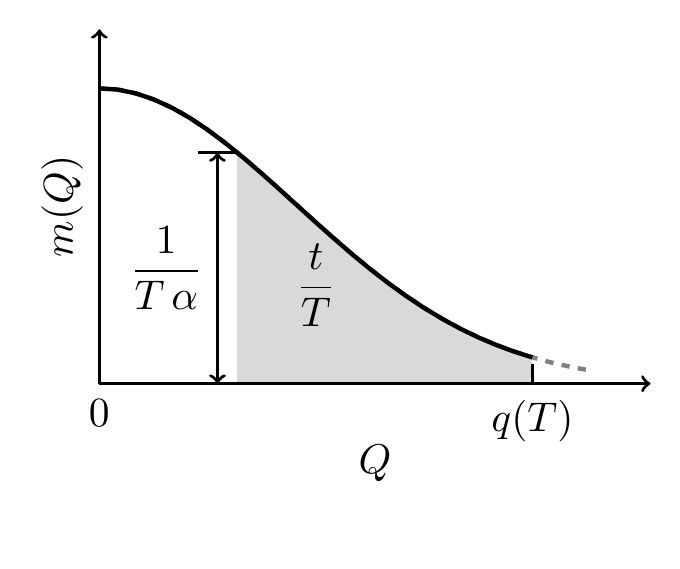
\begin{tikzpicture}[very thick, scale=2.5, every node/.style={scale=1.5}]
    % distribution
    \draw[domain=0:2.5, variable=\x, dashed, gray, ultra thick]
      plot({\x}, {1.5*exp(-0.5*\x*\x)});

    % shade
    \fill [gray!30!white, domain=0.7:2.2, variable=\x]
      (0.7, 0) --
      plot ({\x}, {1.5*exp(-0.5*\x*\x)})
      -- (2.2, 0) -- cycle;

    % thick curve
    \draw[domain=0:2.2, variable=\x, ultra thick]
      plot({\x}, {1.5*exp(-0.5*\x*\x)});

    % label for the shaded area
    \node[] at (1.1, 0.5) {$\dfrac{t}{T}$};

    \draw[<->] (0.6, 0)  --
               node[left, inner sep=1mm]
               {$\dfrac{1}{T \, \alpha}$}
               (0.6, 1.174);
    % label for the ordinate
    %\node[fill=white] at (0.4, 0.7) {$\dfrac{1}{Ta}$};

    \draw[] (0.5, 1.174) -- (0.7, 1.1740);
    \draw[->] (0, 0) -- node[below, inner sep=5mm] {$Q$} (2.8, 0);
    \draw[->] (0, 0) -- node[above, rotate=90] {$m(Q)$} (0, 1.8);

    % xtics
    \draw[] (0.0, 0.1) -- (0.0, 0.0) node[below] {$0$};
    \draw[] (2.2, 0.1) -- (2.2, 0.0) node[below] {$q(T)$};
  \end{tikzpicture}
  %\makebox[\linewidth][c]{
  %  \includegraphics[angle=0, width=0.9\linewidth]{fig/massq.pdf}
  %}
  \caption{
    \label{fig:massq}
    Geometric characterization of the optimal schedule,
    $\alpha(t)$,
    via the normalized mass distribution, $m(Q)$.
    %
    \note{
      The figure was produced by \texttt{tikz}.
      % Gnuplot version by doc/fig/massq.gp
    }%
  }
\end{center}
\end{figure}


Then, from Eq. \eqref{eq:q_opt},
we find that for $Q = q(T) - q(t)$,
%
\begin{align}
  m(Q)
  &=
  \frac{ 1 }
       { T \, \alpha(t) }
  ,
\label{eq:mQ_invTa}
  \\
  \int_Q^{ q(T) }
    m(Q') \, dQ'
  &=
  \frac t T
  ,
\label{eq:intmQ_tT}
\end{align}
%
which means that each point,
$\bigl(t, \alpha(t)\bigr)$,
on the schedule can be mapped
to a point,
$\bigl(Q, m(Q)\bigr)$,
on the mass distribution,
such that the ordinate of the latter curve
gives $1/(T\alpha)$,
and the area under the curve in the domain, $[Q, q(T)]$,
is equal to $t/T$,
as shown in Fig. \ref{fig:massq},

This mapping allows us to classify optimal schedules
as follows.
%
We collect in each class optimal schedules
computed from simulations with the same function, $M(Q)$,
and cutoff value of $q(T)$.
%
The former is determined by the values of
$\lambda_k$'s and $\Gamma_k$'s,
whereas the latter affects the distribution, $m(Q)$,
via the normalization constant, $C$.


In each class, the updating magnitudes of two schedules
of lengths $T_1$ and $T_2$
at corresponding times, $t_1/T_1 = t_2/T_2$,
are related by $T_1 \, \alpha_1(t_1) = T_2 \, \alpha_2(t_2)$.
%
Further, by Eqs.
\eqref{eq:error_asym_Lagrangian}
and
\eqref{eq:Lagrangian_const},
we have
%
\begin{equation}
  \Err_A(T)
  =
  \frac { C^2 } { T }
  =
  \frac 1 T
  \left(
    \int_0^{ q(T) } M(Q) \, dQ
  \right)^2
  ,
\label{eq:error_asym2}
\end{equation}
%
which means that the asymptotic error
is inversely proportional to the simulation length
for schedules in the same class.
%which can be rephrased as another scaling relation
%$$
%T_1 \, \Err_{A1}(T_1) = T_2 \, \Err_{A2}(T_2).
%$$


%The optimal schedule has the following scaling property.
%%
%For two simulations of lengths $T_1$ and $T_2$,
%if $q(T_1) = q(T_2)$
%and they share the same $\lambda_k$'s and $\Gamma_k$'s,
%the updating magnitudes at the corresponding times,
%$t_1/T_1 = t_2/T_2$,
%can be related as $T_1 \, \alpha_1 = T_2 \, \alpha_2$.
%%
%In other words,
%if $\alpha(t_1)$ is
%an optimal schedule of the simulation of length $T_1$,
%then
%$\frac{T_1}{T_2} \alpha\left( \frac{ T_1 } { T_2 } t_2 \right)$
%is an optimal schedule of the simulation of length $T_2$.
%%
%The asymptotic errors are related by
%$T_1 \, E_{A1} = T_2 \, E_{A2}$.



\subsubsection{\label{sec:optinitalpha}
  Optimal initial updating magnitude
}


The above characterization allows us to determine
the optimal initial updating magnitude.
%
Let us now consider simulations in which
the system is initially equilibrated at the same
constant updating magnitude, $a_0$.
%
For these simulations,
we can adjust $q(T)$
to minimize the total error.
%
From Eqs. \eqref{eq:error_res1}
and \eqref{eq:error_asym2},
we find that
the $q(T)$ that minimizes
the total error satisfies
\begin{equation}
  m\bigl( q(T) \bigr)
  =
  \frac{1} { T \, (a_0 / 2) }
  .
\label{eq:opt_qT}
\end{equation}
%
\note{Let $Q_c \equiv q(T)$,
$$
\begin{aligned}
  \frac{
    \partial \Err_R(T)
  }
  {
    \partial Q_c
  }
  &=
  -a_0 \, M^2(Q_c)
  ,
  \\
  \frac{
    \partial \Err_A(T)
  }
  {
    \partial Q_c
  }
  &=
  \frac 2 T \,
  M(Q_c) \,
  \int_0^{ Q_c } M(Q) \, dQ
  .
\end{aligned}
$$
Then solve $\partial (\Err_R + \Err_A) / \partial Q_c = 0$.
}%
By Eqs. \eqref{eq:mQ_invTa} and \eqref{eq:intmQ_tT},
we can rewrite the condition as
\begin{equation}
  \alpha( t = 0 )
  =
  \frac{ a_0 }
       { 2 }
  ,
\label{eq:half_alpha0}
\end{equation}
%
i.e. the optimal initial updating magnitude
is always half of the equilibrium value.
%
This factor, $1/2$,
happens to coincide with the
recommended reduction factor of the updating magnitude
at stage transitions
in the original WL algorithm\cite{
wang2001, *wang2001pre}.


For simulations with the same $a_0$,
the shape of the mass distribution, $m(Q)$,
also determines how much the optimal schedule
would depend on the simulation length, $T$.
%
Since both $M(Q)$ and $m(Q)$ decrease monotonically with $Q$,
Eq. \eqref{eq:opt_qT} shows that
the optimal $q(T)$ increases with
the simulation length, $T$,
more so if $M(Q)$ has a long tail.
%
Thus, if $M(Q)$ decays slowly because of
many near zero eigenvalues, $\lambda_k$'s,
as in the metadynamics case,
both the optimal schedule and
normalized asymptotic error, $\Err_A(T) \cdot T$,
would be sensitive to the simulation length, $T$.
%
In contrast, if all eigenvalues are $1.0$
as in the single-bin or WL updating scheme discussed previously,
the optimal schedule is
given by the universal inverse-time formula,
Eq. \eqref{eq:alpha_invt1},
and the normalized asymptotic error
is roughly a constant
[cf. Eq. \eqref{eq:error_singlebin}].
%
%If $M(Q)$ decays rapidly,
%the distribution $m(Q)$ does not critically
%depend on the cutoff $q(T)$,
%once $q(T)$ is sufficiently large.
%%
%So the optimal schedules of these simulations
%approximately satisfy the scaling relations
%described in Sec. \ref{sec:mass_distr}.
%%
%If, however, $M(Q)$ has a long tail
%because of some near-zero $\lambda_k$'s,
%increasing the simulation length $T$
%generally alters the shape of the optimal schedule.




\subsection{\label{sec:band-matrix}
Homogeneous updating schemes}



Many commonly-used updating schemes
can be characterized by a rigid window
centered on the current bin.
%
We call these schemes homogeneous,
or translationally invariant.
%
An example is the Gaussian updating scheme
used in metadynamics.



\subsubsection{\label{sec:bandkernel}
Updating kernel and eigenvalues}



%While translationally-invariant
%updating schemes
%naturally suit periodic variables\cite{
%dama2014},
%they can also be extended to non-periodic variables
%by imposing the reflective boundary condition\cite{
%bussi2006}.
%%
%For simplicity, we will assume that the target
%distribution is flat, or $p_i = 1/n$, below.



%It is natural to first introduce homogeneous updating schemes
For a periodic variable\cite{dama2014},
the updating matrix, $\mathbf w$,
assumes the following form
%
\begin{equation}
  w_{ij}
  =
  \mu_{i-j}
  +
  \mu_{i-j+n}
  +
  \mu_{i-j-n}
  ,
\notag
%\label{eq:w_band_pbc}
\end{equation}
%
where
$\mu_{-b}, \dots, \mu_b$ ($b \le n/2$)
are a set of numbers satisfying
%
\begin{equation}
  \mu_{-b} + \cdots + \mu_b = 1
  ,
\label{eq:mu_normalization}
\end{equation}
%
and $\mu_l = 0$ for $|l| > b$.
%
We will further impose the symmetry
%
\begin{equation}
  \mu_i = \mu_{-i}
  .
\label{eq:mu_symm}
\end{equation}
%
If $b = n/2$, then $\mu_{-b}$ is removed
from the sum in Eq. \eqref{eq:mu_normalization}
to avoid double counting.
%
These numbers constitute an \emph{updating kernel}\cite{bussi2006}.
%
In this way, the matrix, $\mathbf w$,
being symmetric with respect to the indices, $i$ and $j$,
satisfies Eqs. \eqref{eq:w_sumj}-\eqref{eq:w_balance},
for the flat distribution.


To find the eigenvectors,
we define, for a periodic variable, $\phi_i$,
the out-of-boundary values by
%
\begin{equation}
  \phi_i = \phi_{i \pm n},
\label{eq:phi_pbc}
\end{equation}
%
such that $i \pm n$ lies in between $1$ and $n$.
%
Then, the multiplication of the matrix, $\mathbf w$,
is equivalent to a convolution with the kernel:
%
\begin{equation}
  \sum_{ j = 1 }^n
    w_{ij} \, \phi_j
  =
  \sum_{ j = 1 - n }^{ 2 \, n }
    \mu_{i - j} \, \phi_j
  =
  \sum_{ l = -b }^{ b }
    \mu_l \, \phi_{ i - l}
  .
\label{eq:wmul_to_convol}
\end{equation}
%
\note{The derivation of the first step of
  Eq. \eqref{eq:wmul_to_convol}:
$$
\begin{aligned}
  \sum_{j = 1}^n
    w_{ij} \, \phi_j
  &=
  \sum_{j = 1}^n
    \mu_{i - j} \, \phi_j
  +
  \sum_{j = 1}^n
    \mu_{i - j - n} \, \phi_j
  +
  \sum_{j = 1}^n
    \mu_{i - j + n} \, \phi_j
  \\
  &=
  \sum_{j = 1}^n
    \mu_{i - j} \, \phi_j
  +
  \sum_{l = 1+n}^{2 \, n}
    \mu_{i - l} \, \phi_{l - n}
  +
  \sum_{l = 1-n}^0
    \mu_{i - l} \, \phi_{l + n}
  \\
  &=
  \sum_{j = 1}^n
    \mu_{i - j} \, \phi_j
  +
  \sum_{l = 1+n}^{2 \, n}
    \mu_{i - l} \, \phi_{l}
  +
  \sum_{l = 1-n}^0
    \mu_{i - l} \, \phi_{l}
  \\
  &=
  \sum_{j = 1-n}^{2 \, n}
    \mu_{i - j} \, \phi_j
  .
\end{aligned}
$$
The second step of Eq. \eqref{eq:wmul_to_convol}
follows from the constraint, $\mu_l = 0$, for $|l| > b$.

Similarly,
for the left eigenvector, we have
$$
  \sum_{ i = 1 }^n
    \phi_i \, w_{ij}
  =
  \sum_{ l = -b }^b
    \phi_{j - l} \, \mu_{-l}
  .
$$
But due to the symmetry Eq. \eqref{eq:mu_symm},
it is identical to \eqref{eq:wmul_to_convol}.
}
%
As a result, the characteristic equation,
$\mathbf w \, \pmb\phi = \lambda \, \pmb\phi$,
can be solved by discrete Fourier transform.
%
We may construct a set of orthonormal eigenvectors,
$\pmb\phi^{(1)}, \dots, \pmb\phi^{(n)}$,
compatible with the periodicity, Eq. \eqref{eq:phi_pbc},
%
\begin{equation}
  \phi^{(k)}_j
  =
  \phi_{kj}
  =
  \frac 1 n
  \exp
  \left[
    \ii
    \frac{ (k - 1) \, j \, 2 \, \pi }
         {            n             }
  \right]
  ,
  \notag
\end{equation}
%
where $\ii^2 = -1$, and
the eigenvalues are
the Fourier or cosine transform of the updating kernel:
%
\begin{equation}
  \lambda_k
  =
  \mu_0
  +
  2 \,
  \sum_{ l = 1 }^b
  \mu_l
  \cos
  \frac{ (k - 1) \, l \, 2 \, \pi }
       {            n             }
  .
  \label{eq:wband_eigenvalue_pbc}
\end{equation}
%
\note{Consider the unnormalized version
  $$
  \Phi^{(k)}_j =
  \exp\left[
    \frac{ ( k - 1 ) \, j \, 2 \, \pi }
         {              n             }
    \ii
  \right]
  ,
  $$
  we have
  $$
  \begin{aligned}
  \sum_{j = 1}^n
    w_{ij} \, \Phi^{(k)}_j
  &=
  \sum_{l = -b}^b
    \mu_l \, \Phi^{(k)}_{i - l}
  \\
  &=
  \mu_0 \, \Phi^{(k)}_i
  +
  \sum_{l = 1}^b
    \mu_l \,
    \left[ \Phi^{(k)}_{i - l} + \Phi^{(k)}_{i + l} \right]
  \\
  &=
  \Phi^{(k)}_i \,
  \left[
    \mu_0
    +
    2 \sum_{l = 1}^b
      \mu_l \, \cos
      \frac{ (k - 1) \, l \, 2 \, \pi }
           {            n             }
  \right]
  .
  \end{aligned}
  $$
  The term in the square brackets is the eigenvalue given by
  Eq. \eqref{eq:wband_eigenvalue_pbc}.
}
%
Note, however, the two-fold degeneracy as
$\lambda_{n - k + 2} = \lambda_k$.



To adapt the above formulae to a non-periodic variable,
we use the reflective boundary condition\cite{bussi2006},
and change the form of the updating matrix to
%
%
\begin{equation}
  w_{ij}
  =
  \mu_{ i - j }
  +
  \mu_{ i + j - 1 }
  +
  \mu_{ i + j - 2 n - 1 }
  ,
  \label{eq:w_band_refl}
\end{equation}
%
where the last two terms on the right hand side,
representing two reflective mirrors at
$j = 1/2$ and $j = n + 1/2$,
are added to avoid unintended distortion\cite{dickson2011, mcgovern2013}
to the equilibrium distribution\cite{bussi2006},
such that Eqs. \eqref{eq:w_sumj}-\eqref{eq:w_balance}
are satisfied.
%
Again, the updating kernel should satisfy
Eqs. \eqref{eq:mu_normalization}
and \eqref{eq:mu_symm},
but
the cutoff $b$ only needs to be less than $n$.

Parallel to Eq. \eqref{eq:phi_pbc},
we define the out-of-boundary values
of $\phi_i$ as
%
\begin{equation}
  \phi_i
  =
  \begin{dcases}
    \phi_{ 1 - i }           & \mathrm{for \;} i \le 0, \\
    \phi_{ 2 \, n + 1 - i }  & \mathrm{for \;} i > n,
  \end{dcases}
\label{eq:phi_refl}
\end{equation}
%
such that the matrix multiplication is still equivalent to
a convolution as Eq. \eqref{eq:wmul_to_convol}.
%
\note{The derivation of Eq. \eqref{eq:wmul_to_convol}
  in this case is similar,
  $$
  \begin{aligned}
    \sum_{j = 1}^n w_{ij} \, \phi_j
    &=
    \sum_{j = 1}^n
      \mu_{i - j} \, \phi_j
    +
    \sum_{j = 1}^n
      \mu_{i + j - 1} \, \phi_j
    +
    \sum_{j = 1}^n
      \mu_{i + j - 2 \, n - 1} \, \phi_j
    \\
    &=
    \sum_{j = 1}^n
      \mu_{i - j} \, \phi_j
    +
    \sum_{l = 1 - n}^0
      \mu_{i - l} \, \phi_l
    +
    \sum_{l = n + 1}^{ 2 \, n }
      \mu_{i - l} \, \phi_l
    \\
    &=
    \sum_{j = 1 - n}^{ 2 \, n}
      \mu_{i - j} \, \phi_j.
  \end{aligned}
  $$
}%
We note that Eq. \eqref{eq:phi_refl}
defines a periodic variable of period $2 \, n$
with a reflective symmetry around $i = 1/2$.
%
Accordingly, the eigenvectors,
$\pmb\phi^{(1)}, \dots, \pmb\phi^{(n)}$,
must share the same periodicity,
and be even functions about the axis, $i = 1/2$:
%
\begin{equation}
  \phi^{(k)}_i
  =
  \phi_{k i}
  =
  \frac{ \sqrt{ 2 - \delta_{k, 1} } }
       {             n              }
  \cos \frac{ ( k - 1) \, \left( i - \frac 1 2 \right) \, 2 \, \pi}
            {                    2 \, n                           }
  ,
\notag
%\label{eq:wband_eigenvector_refl}
\end{equation}
%
The eigenvalues can be borrowed from
Eq. \eqref{eq:wband_eigenvalue_pbc},
with the period, $n$, doubled:
%
\begin{align}
  \lambda_k
  &=
  \mu_0
  +
  2
  \sum_{l = 1}^b
    \mu_l
    \cos \frac{(k - 1)  \, l \, 2 \, \pi}{ 2 \, n }
  .
\label{eq:wband_eigenvalue_refl}
\end{align}
%
\note{Derivation.
  First consider the unnormalized eigenvectors,
  $$
  \Phi^{(k)}_i
  =
  \cos \frac{ \left( i - \frac 1 2 \right) (k - 1) \, \pi}{n},
  $$
  which satisfies Eq. \eqref{eq:phi_refl}.
  %
  So, by Eq. \eqref{eq:wmul_to_convol},
  $$
  \begin{aligned}
  \sum_{i = 1}^n
    \Phi^{(k)}_i \, w_{ij}
  &=
  \sum_{l = -b}^b
    \Phi^{(k)}_{j - l} \, \mu_l
  \\
  &=
    \Phi^{(k)}_j \, \mu_0
  + \sum_{l=0}^{b}
    \mu_l \,
    \left[
      \Phi^{(k)}_{j-l}
      +
      \Phi^{(k)}_{j+l}
    \right]
  \\
  &= \Phi^{(k)}_j \, \lambda_k,
  \end{aligned}
  $$
  with $\lambda_k$ given by Eq. \eqref{eq:wband_eigenvalue_refl}.
}%
%
We may unify Eqs. \eqref{eq:wband_eigenvalue_refl}
and \eqref{eq:wband_eigenvalue_pbc} as
%
\begin{equation}
  \lambda_k
  =
  \mu_0
  +
  2
  \sum_{ l = 1 }^b
    \mu_l \,
    \cos \frac{ (k - 1) \, l \, g \, \pi }
              {            n             }
  ,
  \label{eq:wband_eigenvalue}
\end{equation}
%
where the degeneracy, $g$, is $2$
for the periodic case,
or $1$ otherwise.
%
In both cases,
the eigenvalues, $\lambda_k$'s,
are the cosine transform of
the updating kernel.

For the updating scheme to be stable,
the cosine transform of the kernel
must be nonnegative.
%
If this is not so,
we can modify the kernel
using the technique described
in Appendix \ref{sec:stabilize_wband}.

We discuss two special cases below.



\subsubsection{\label{sec:nnscheme}
Triple-bin updating scheme}



If $\mu_2 = \dots = \mu_b = 0$,
the matrix, $\mathbf w$, is tridiagonal,
%%
%\begin{equation}
%\arraycolsep=3.6pt\def\arraystretch{1.4}
%\mathbf w
%=
%\left(
%  \begin{array}{cccccccc}
%    1 - \mu_1   & \mu_1 & 0 & \dots & 0 \\
%    \mu_1 & 1 - 2 \, \mu_1  & \mu_1 & \dots & 0 \\
%    \vdots & &  & & \vdots \\
%    0 & \dots & \mu_1 & 1 - 2 \, \mu_1  & \mu_1 \\
%    0 & \dots & 0 & \mu_1 & 1 - \mu_1
%  \end{array}
%\right).
%\label{eq:wnn}
%\end{equation}
%%
%We have
and the eigenvalues are
\begin{equation}
  \lambda_k
  =
  1 -
  4 \, \mu_1 \sin^2
  \frac{ (k - 1) \, g \, \pi }
       {       2 \, n        }
  .
\notag
%\label{eq:wnn_eigenvalue}
\end{equation}
%
So this updating scheme is stable if
$\min \lambda_k \ge 0$,
or
\begin{equation}
  \mu_1 \le
  \begin{dcases}
    \frac 1 4
    & \mathrm{periodic \; and \;} n \mathrm{ \; even,}
    \\
    \frac 1 4
    \sec^2
    \left( \frac{  \pi   }
                { 2 \, n }
    \right)
    & \mathrm{otherwise}.
  \end{dcases}
\notag
%\label{eq:nn_stable}
\end{equation}

\note{
If the variable is periodic ($g = 2$) and $n$ is even,
the minimum is achieved at $k = n/2$.

If the variable is periodic ($g = 2$) but $n$ is odd,
the minimum is achieved at $k = (n+1)/2$.
$$
\sin^2\left(
  \frac{n-1}{2n} \pi
\right)
=
\cos^2\left(
  \frac{\pi}{2n}
\right)
.
$$

If the variable is nonperiodic ($g = 1$)
the minimum is achieved at $k = n$.
}





\subsubsection{Gaussian updating scheme}



We define a Gaussian updating scheme
as an updating scheme with a
Gaussian-shaped kernel.
%
This updating scheme is commonly
used in metadynamics.
%
Below we show its stability
in the continuous limit.



For $n \gg 1$,
we define
$x = l \, \Delta x$,
and
$\mu_l = \mu(x) \, \Delta x$,
where
$\Delta x = g \, \pi/n$
is the bin size.
%
By assuming the largest cutoff, $b \approx n/g$,
we can approximate Eq. \eqref{eq:wband_eigenvalue}
as an integral:
%
\begin{equation}
  \lambda_k
  =
  2 \int_0^\pi
    \mu(x) \, \cos \bigl[ (k-1) \, x \bigr] \, dx,
\notag
%\label{eq:lambda_int}
\end{equation}
%
with the normalization
%
$
  1 = 2 \int_0^\pi \mu(x) \, dx.
$
\note{
\begin{align*}
  \lambda_k
  &\approx
  \int_0^b \mu_l \, \cos[(k-1) \, x] \, dl
  \\
  &=
  \int_0^b \mu(x) \, \cos[(k-1) \, x] \, \Delta x \, dl
  \\
  &=
  \int_0^{b \, \Delta x} \mu(x) \, \cos[(k-1) \, x] \, dx
\end{align*}
The upper limit,
$b \, \Delta x \approx (n/g) \, (g\,\pi/n) = \pi$.
}

For the Gaussian updating kernel,
if the width, $\sigma$, satisfies $\Delta x \ll \sigma \ll 1$,
we can extend
the upper limit of the integrals
to infinity, and
%
\begin{equation}
  \mu(x)
  =
  \frac{            1            }
       { \sqrt{ 2 \pi \sigma^2 } }
  %
  \exp\left(
        -\frac{       x^2     }
              { 2 \, \sigma^2 }
      \right)
  .
\notag
\end{equation}
%
%
If follows that all eigenvalues are positive\cite{bussi2006}:
%
\begin{align}
  \lambda_k
  &=
  \exp\left[
        -\frac{ (k - 1)^2 \, \sigma^2 }
              {           2           }
      \right]
  %\notag
  %\\
  %&=
  %\exp\left[
  %      -\frac{ \pi^2 }{ 2 }
  %      \left(
  %        \frac{ k - 1 }
  %             {   n   }
  %      \right)^2
  %      \left(
  %        \frac{  \sigma }
  %             { \Delta x }
  %      \right)^2
  %    \right]
  .
\notag
%\label{eq:lambda_Gaussian}
\end{align}



%However,
%as $\sigma/\Delta x \gg 1$,
%the smallest eigenvalue
%%
%$$
%\lambda_n
%\approx
%\exp\left(
%      -\frac{ n^2 \, \sigma^2 }
%            {        2        }
%    \right)
%=
%\exp\left[
%      -\frac{ \pi^2 }{ 2 }
%      \left(
%        \frac{  \sigma }
%             { \Delta x }
%      \right)^2
%    \right]
%.
%$$
%%
%is exponentially small.
%%
%This means that
%the optimal value of $\lambda$
%given by Eq. \eqref{eq:optimal_lambda_approx}
%would be too small in practice,
%for it requires $\lambda < 2 \, \lambda_n$.
%%
%In other words,
%with a reasonable $\lambda$,
%the error of the last few fluctuation modes
%will always decay suboptimally,
%accordingly to Eq. \eqref{eq:error_asym_invt}.
%%
%However, since these modes
%represent short wavelength fluctuations,
%and these modes may be in
%the system under consideration.
%%
%Thus,
%we can truncate the sum of the error function
%in Eq. \eqref{eq:error_asym_invt}
%at some $k_{\max}$,
%which corresponds to a minimal length scale
%$l_{\min} = \Delta x \, (n /k_{\max}) = \pi/k_{\max}$
%greater than $\sigma$.
%%
%Then,
%$$
%\lambda_{ k_{\max} }
%\approx
%\exp\left(
%      -\frac{ k_{\max}^2 \, \sigma^2 }
%            {           2            }
%    \right)
%=
%\exp\left(
%      -\frac{  \pi^2 \, \sigma^2    }
%            {    2 \, l_{\min}^2  }
%    \right).
%$$



\subsubsection{\label{sec:invert_wband}
Inversion}



Since the eigenvalues are related to the updating kernel
by a cosine transform,
Eq. \eqref{eq:wband_eigenvalue},
the relation can be readily inverted.
%
In the periodic case,
we have
%the inversion formula is
%
\begin{equation}
  \mu_l
  =
  \frac 1 n
  \sum_{ k = 1 }^n
  \lambda_k
  \cos \frac{ (k - 1) \, l \, 2 \, \pi }
            {            n             }
  .
\label{eq:mu_from_lambda_pbc}
\end{equation}


In the non-periodic case,
the formula is
%
\begin{align}
  \mu_l
  =
  \frac 1 { 2 \, n }
  \sum_{ k = 1 }^{ 2 \, n }
    \lambda_{ k } \,
    \cos \frac{ (k - 1) \, l \, \pi }
              {            n        }
  ,
\label{eq:mu_from_lambda_refl}
\end{align}
%
where
we have defined
$\lambda_k \equiv \lambda_{2 \, n + 2 - k}$
for $k = n + 2, \dots, 2 \, n$,
as well as
%
\begin{align}
  \lambda_{ n + 1 }
  =
  (-1)^{ n - 1 }
  \lambda_1
  +
  2 \, \sum_{ k = 2 }^{ n }
      (-1)^{n - k} \, \lambda_k
  ,
\label{eq:lambdan}
\end{align}
to satisfy the constraint, $\mu_n = 0$.
%
\note{Eq. \eqref{eq:lambdan}
  ensures that the $\mu_n$
  computed from Eq. \eqref{eq:mu_from_lambda_refl}
  vanishes.

  %The inversion formula is derived from the cosine transform.
  %
  If we define $\mu_n = 0$ and
  %
  $
    \mu_{ 2 n - l } = \mu_l,
  $
  for
  $l = 1, \dots, n - 1$,
  %
  then Eq. \eqref{eq:wband_eigenvalue_refl} can be rewritten as
  %
  \begin{align}
    \lambda_{k+1}
    =
    \sum_{ l = 0 }^{ 2 \, n - 1 }
    \mu_l \, \cos \frac{ k \, l \, \pi } { n }.
  \notag
  %\label{eq:lambda_cosine_sum}
  \end{align}
  %
  This formula for $\lambda_{k+1}$
  can be readily extended to $k = 2 \, n - 1$,
  and we have
  %
  $
    \lambda_{ 2 \, n + 2 - k } = \lambda_k
    .
  $
  %
  Thus,
  %
  $$
  \begin{aligned}
    \sum_{ k = 0 }^{ 2 \, n - 1 }
      \lambda_{ k + 1 } \,
      \cos \frac{ k \, p \, \pi }
                {      n        }
    &=
    \sum_{ k = 0 }^{ 2 \, n - 1 }
      \sum_{ l = 0 }^{ 2 \, n - 1 }
        \mu_l \,
        \cos \frac{ k \, l \, \pi }
                  {      n        }
        \cos \frac{ k \, p \, \pi }
                  {      n        }
    \\
    &=
    \sum_{ l = 0 }^{ 2 \, n - 1 }
      \frac{ \mu_l } { 2 }
      \sum_{ k = 0 }^{ 2 \, n - 1 }
        \cos \frac{ k \, (p + l) \, \pi }
                  {      n        }
                  +
        \cos \frac{ k \, (p - l) \, \pi }
                  {      n        }
    \\
    &=
    \sum_{ l = 0 }^{ 2 \, n - 1 }
      \mu_l \, n \left(
        \delta_{ p + l - 2 \, n, 0 }
        +
        \delta_{ p - l, 0 }
      \right)
    \\
    &=
    n \, \left( \mu_p + \mu_{ 2 \, n - p} \right)
    =
    2 \, n \, \mu_p.
  \end{aligned}
  $$
  This entails Eq. \eqref{eq:mu_from_lambda_refl}.
  %
  The value of $\lambda_{n + 1}$
  can be deduced from
  imposing $\mu_n = 0$
  and solving Eq. \eqref{eq:mu_from_lambda_refl}
  for $l = n$,
  yielding Eq. \eqref{eq:lambdan}.
}



\subsection{\label{sec:cmpschemes}
Comparison of updating schemes}


Now that we can compute the optimal schedule
for a given updating scheme,
we will turn to the problem of finding
optimal updating schemes below.


\subsubsection{\label{sec:optWL}
Asymptotic optimality of the single-bin scheme}



We will first show
that the single-bin scheme is asymptotically optimal.
%
Consider a class of $\mathbf w$ matrices
sharing the same set of eigenvectors,
hence the same $\Gamma_k$'s,
but with different positive eigenvalues,
$\lambda_k$'s.
%
Using the Cauchy-Schwarz inequality, we have,
for any set of nonnegative numbers, $c_k$'s,
%
\begin{align}
&
\left(
  \int_0^T dt
    \sum_{k = 2}^n
      \Gamma_k \, \dot u_k^2\bigl( q(t) \bigr)
\right)
%
\left(
  \int_0^T dt
    \sum_{k = 2}^n
      \Gamma_k \, c_k^2
\right)
%
\notag
\\
&
\qquad \qquad
\ge
\left(
  \int_0^T dt
    \sum_{k = 2}^n
      \Gamma_k \, c_k \, \dot u_k \, \bigl( q(t) \bigr)
\right)^2
\notag
\\
&
\qquad \qquad
=
\left(
  \sum_{k = 2}^n \Gamma_k \, c_k
    \left[
      1 - e^{ -\lambda_k \, q(T) }
    \right]
\right)^2.
\label{eq:CSineq}
\end{align}
%
%\note{
This inequality follows from the non-negativity of
the quadratic polynomial,
$$
\int_0^T
  dt \sum_{k = 2}^n \Gamma_k \,
    \left( \dot u_k \, \chi - c_k \right)^2
  \equiv
  A_2 \, \chi^2 + A_1 \, \chi + A_0
  ,
$$
which must carry a non-positive discriminant:
$A_1^2 - 4 \, A_0 \, A_2 \le 0$.
%}%
%
Note that the last expression of Eq. \eqref{eq:CSineq}
depends on the curve, $q(t)$ ($0 < t < T$),
only through the endpoint value, $q(T)$,
which is fixed in the variational process.
%
Thus, the inequality sets a lower bound
for the asymptotic error $\Err(T)$
given in Eq. \eqref{eq:error_asym1}.
%
The equality is achieved
if $\dot u_k\left( q(t) \right) = c_k$
for all $k = 2, \dots, n$ at any $t$,
up to a multiplicative factor.
%
Solving these equations yields
%
\begin{equation}
  \alpha(t) = \frac{              1             }
                   { \lambda_k \, (t + t_{k0} ) },
\label{eq:alpha_invtk}
\end{equation}
with
\begin{equation}
  t_{k0} = \frac{             T            }
                { e^{ \lambda_k q(T) } - 1 }.
\label{eq:tk0}
\end{equation}
%
\note{Derivation.
  Integrating $\dot u_k = c_k$ yields
  \begin{equation}
    u_k(t) = c_k \left(t + t_{k0} \right).
  \tag{UK}
  \label{neq:ui_solution}
  \end{equation}
  Given that $u_k(T) = 1$ and $u_k(0) = e^{-\lambda_k \, q(T)}$,
  we have
  $$
  c_k = \frac{ 1 }{ T + t_{k0} },
  \quad
  \mathrm{and\;}
  \frac{ t_{k0} } { T + t_{k0} }
  =
  e^{ -\lambda_k \, q(T) }.
  $$
  Taking the logarithm of Eq. \eqref{neq:ui_solution} yields
  $$
  -\lambda_k \, q(T) + \lambda_k \, q(t)
  = \ln c_k + \ln \left( t + t_{k0} \right).
  $$
  Differentiating this with respect to $t$ yields
  Eq. \eqref{eq:alpha_invtk}.
}
%
Such a solution is possible only if
all nontrivial eigenvalues are the same
%
\begin{equation}
  \lambda_2 = \dots = \lambda_n.
  \notag
\end{equation}
%
Then, by Eq. \eqref{eq:tk0},
all $t_{k0}$'s also share the same value,
$t_0$,
such that
$u_k = (t + t_0) / (T + t_0)$,
and
$c_k = 1/(T + t_0)$
for $k \ge 2$.
%
The asymptotic error is then
%
\begin{align}
  \Err_A(T)
  =
  \frac{       T     }
       { (T + t_0)^2 }
  \sum_{ k = 2 }^n
    \Gamma_k
  .
\label{eq:error_asym_singlebin}
\end{align}
%
If we further assume $\lambda_2 = \cdots = \lambda_n = 1$,
%the optimal schedule given by
Eq. \eqref{eq:alpha_invtk}
recovers Eq. \eqref{eq:alpha_invt1}.
%

Since the first eigenmode represents
a uniform shift of the bias potential,
we can freely set $\lambda_1$ to be the same as $\lambda_2$
without changing the nature of the updating scheme.
%
Note, an updating matrix
with identical eigenvalues
is a multiple of the identity matrix.
%
Thus,
the corresponding updating scheme,
the single-bin scheme, is most efficient
in asymptotic convergence.
%if no eigenvalue $\lambda_k$ is zero.
%
In Appendix \ref{sec:upperbound},
we will show that the opposite limit of
a set of well-separated eigenvalues
will provide an upper bound for
the asymptotic error, Eq. \eqref{eq:error_asym_ubound}.



\subsubsection{\label{sec:optscheme}
Bandpass updating schemes}


We can generalize
the single-bin scheme to a class of
perfect (brick-wall) \emph{bandpass} updating schemes
that ignore short-wavelength eigenmodes,
which are typically local noise.
%
Mathematically, these updating schemes will have
zero eigenvalues for the ignored modes,
and they are useful if we can assume that
the ignored modes are absent from the PMF.
%
For example,
%if we can assume
by assuming
that the PMF is sufficiently smooth
such that the eigenmodes can be limited to $k \le K$,
%
we can construct an updating scheme with
$$
\lambda_1 = \cdots = \lambda_K = 1,
\mathrm{\; and \;}
\lambda_{K+1} = \cdots = \lambda_n = 0.
$$
%
Then,
we can change the upper limit of the sum in
Eq. \eqref{eq:error_asym_singlebin} to $K$:
%
%Then,
%Eq. \eqref{eq:error_singlebin} is changed to
%
\begin{equation}
  \Err_A(T)
  =
  \frac {       T     }
        { (T + t_0)^2 }
  \sum_{ k = 2 }^K
    \Gamma_k.
%\notag
\label{eq:error_asym_sinc}
\end{equation}
%
The optimal schedule of these schemes
remains to be the inverse-time schedule
given by Eq. \eqref{eq:alpha_invt1}.
%
Below, we construct these schemes for
the homogeneous case.
%
The definition of the cutoff, $K$, will be modified
for mathematical convenience.

For a periodic variable, we demand
%
$$
\begin{aligned}
&
\lambda_1 = \cdots = \lambda_{K+1}
= \lambda_{n-K+1} = \cdots = \lambda_n = 1,
\\
&
\lambda_{K+2} = \cdots = \lambda_{n-K} = 0,
\end{aligned}
$$
for $K \ge 1$.
%
Then by using
Eq. \eqref{eq:mu_from_lambda_pbc},
we get
\begin{equation}
  \mu_l
  =
  \frac{
    \sin
    \dfrac{ (2 K + 1) \, l \, \pi }
         {              n        }
  }
  {
    n \, \sin \dfrac{ l \, \pi } { n }
  }
  .
\notag
%\label{eq:mu_sinc_pbc}
\end{equation}
\note{Derivation.
$$
\begin{aligned}
\mu_l
&=
\frac 1 n \sum_{k = 0}^{n-1} \lambda_{k+1} \cos \frac{ k \, l \, 2 \, \pi } { n }
\\
&=
\frac{1}{n}
\left(
  1 +
  \sum_{k=1}^K
  \cos \frac { k \, l \, 2 \, \pi } { n }
  +
  \sum_{k=n-K}^{n-1}
  \cos \frac { k \, l \, 2 \, \pi } { n }
\right)
\\
&=
\frac 1 n
\sum_{k=-K}^K
\cos \frac { k \, l \, 2 \, \pi } { n }
=
  \frac{
    \sin
    \dfrac{ (2 K + 1) \, l \, \pi }
         {              n        }
  }
  {
    n \, \sin \dfrac{ l \, \pi } { n }
  }
.
\end{aligned}
$$
}

For a non-periodic variable, we demand
$$
\lambda_1 = \cdots = \lambda_{K+1} = 1,
\qquad
\lambda_{K+2} = \cdots = \lambda_n = 0.
$$
Then Eq. \eqref{eq:lambdan} gives
$\lambda_{n+1} = (-1)^{n+K-1}$,
and from Eq. \eqref{eq:mu_from_lambda_refl},
we have
\begin{equation}
  \mu_l
  =
  \frac{1}{2 \, n}
  \left[
    (-1)^{n+K+l-1}
    +
    \frac{
      \sin
      \dfrac{ (2 K + 1) \, l \, \pi }
           {         2 \, n        }
    }
    {
      \sin \dfrac{ l \, \pi } { 2 \, n }
    }
  \right]
  .
\label{eq:mu_sinc_refl}
\end{equation}
\note{Derivation.
$$
\begin{aligned}
  \lambda_{n+1}
  &=
  (-1)^{n-1}
  \left[
    \lambda_1
    - 2 \, \lambda_2
    + 2 \, \lambda_3 - \cdots
    + (-1)^{K} 2 \, \lambda_{K+1})
  \right]
  \\
  &=
  \begin{dcases}
    (-1)^{n-1} & K \mathrm{\; even,} \\
    (-1)^n     & K \mathrm{\; odd.}
  \end{dcases}
\end{aligned}
$$
So
$$
\begin{aligned}
  \mu_l
  &=
  \frac{1}{2\,n}
  \left[
    1 +
    2 \sum_{k=2}^{K+1}
    \cos \frac { (k - 1) \, l \pi } { n }
    +
    (-1)^{n+K-1} (-1)^l
  \right]
  \\
  &=
  \frac{1}{2\,n}
  \left[
    (-1)^{n+K+l-1}
    +
    \sum_{k=-K}^{K}
    \cos \frac { k \, l \pi } { n }
  \right]
  .
\end{aligned}
$$
}%


\begin{figure}[h]
\begin{center}
  \makebox[\linewidth][c]{
    \includegraphics[angle=0, width=0.95\linewidth]{fig/sinc.pdf}
  }
  \caption{
    \label{fig:sinc}
    Updating kernels of the bandpass updating schemes
    compared to a Gaussian with a similar width.
    %
    The lines are a guide to the eyes.
    Inset. Updating matrix in the non-periodic case.
    %
    \note{This figure was produced by \texttt{doc/fig/sinc.gp}.
      The data were computed by the program \texttt{prog/predict},
      see particularly the function \texttt{intq\_save()}
      in \texttt{prog/intq.h} for panel (a),
      and the functions \texttt{savewin()}
      and \texttt{savewinmat()}
      in \texttt{prog/invt.h} for panel (b),
      The data were saved under the directory \texttt{data/sinc}.
      See the \texttt{make} object \texttt{sincsingle}
      in the \texttt{Makefile} there.
    }%
  }
\end{center}
\end{figure}


In Fig. \ref{fig:sinc},
we give examples of the updating kernels
of the bandpass updating schemes,
compared to a Gaussian
with a similar width, $\sigma$,
%
\begin{equation}
  \sigma
  \approx
  \frac
  {
    n
  }
  {
    \sqrt{ 2 \, \pi } \, g \, K
  }
  .
\label{eq:sigma_equiv}
\end{equation}
%
%where $g = 2$ for the periodic case
%or $g = 1$ otherwise.
%
The kernel in the non-periodic case is a sawtooth
because of the term, $(-1)^{n+K+l-1}$,
in Eq. \eqref{eq:mu_sinc_refl}.
%
However, as shown in the inset, % of Fig. \ref{fig:sinc}(b),
the ruggedness disappears
in the updating matrix by Eq. \eqref{eq:w_band_refl},
as the above oscillatory term for $l = i - j$
is canceled by the term for either $l = i + j - 1$
or $l = i + j - 2 \, n - 1$
with the opposite sign.



\subsubsection{\label{sec:finlencorr}
Finite-length correction}



In the above section,
we have focused on
the asymptotic error.
%
By including the residual error
and minimizing the total error,
we get the optimal $t_0$,
which is, according to Eq. \eqref{eq:half_alpha0},
%
%%Assuming the system is initially equilibrated
%%under a constant updating magnitude,
%%$a_0$,
%Assuming Eq. \eqref{eq:error_res1} with
%$$
%q(T)
%=
%\int_0^T \frac{ dt } { t + t_0 }
%=
%\ln \frac{ T + t_0 } { t_0 }.
%$$
%%
%we have, from Eqs. \eqref{eq:error_split}
%and \eqref{eq:error_asym_sinc},
%%
%\begin{equation}
%  \Err
%  =
%  \Err_R + \Err_A
%  =
%  \frac { \frac 1 2 a_0 \, t_0^2 + T }
%        {          ( T + t_0 )^2          }
%  \sum_{ k = 2 }^K \Gamma_k
%  .
%\notag
%%\label{eq:error_sinc0}
%\end{equation}
%%
%The minimum is reached at
%
\begin{equation}
  t_0
  =
  \frac{  2  }
       { a_0 }
  .
\label{eq:t0_sinc}
\end{equation}
%
For the single-bin updating scheme,
it recovers Eq. \eqref{eq:t0_singlebin}
under the assumption of Eq. \eqref{eq:y2_eql}.
%
From Eqs. \eqref{eq:error_split},
\eqref{eq:error_res1},
\eqref{eq:tk0},
and
\eqref{eq:error_asym_sinc},
we get
%
\begin{equation}
  \Err(T)
  =
  \frac{   1     }
       { T + t_0 }
  \sum_{ k = 2 }^K
    \Gamma_k
  .
\label{eq:error_sinc}
\end{equation}
%
which serves as a generalization of
the result from the single-bin scheme, Eq. \eqref{eq:Emin_singlebin}.
%
This error decreases with increasing simulation length,
as one would expect from an equilibrium FDS simulation.
%In Appendix \ref{sec:equilerr},
%we show that the above error tends
%to the error of the ideal equilibrium FDS simulation
%in the asymptotic limit.





%
%For example, consider a system that is initially
%prepared under a fixed $a_0$
%at the beginning of the schedule $\alpha(t)$.
%%
%Then for shorter times, $T \approx 0$,
%the error, dominated by the residual error
%given by Eq. \eqref{eq:error_res1},
%is clearly smaller if some eigenvalues
%are less than $1.0$ (the single-bin case).
%
%In practice, real simulations
%may have long achieved the desired precision
%before reaching the asymptotic regime,
%especially if the updating matrix
%has some $\lambda_k$'s close to $0$.




\section{\label{sec:results}
Numerical results}



We tested the above theory on a model system
described in Sec. \ref{sec:results_system}.
%
We verify the method of computing errors
%using an inverse-time schedule
in Sec. \ref{sec:results_invt}
%
and study the optimal schedule from
Eq. \eqref{eq:q_opt}
in Sec. \ref{sec:results_optschedule}.
%
Finally, we compare the Gaussian and
bandpass updating schemes %of different widths
in Sec. \ref{sec:results_cmpschemes}.



\subsection{\label{sec:results_system}
Test system and simulation protocol}



Our test system is a one-dimensional model system, in which
$i$ represents a non-periodic variable,
and $n = 100$.
%
Both the target and intrinsic distributions
are assumed to be flat:
$p^*_i = p_i = 1/n$,
along with the distribution, $\rho_i$, in Eqs.
\eqref{eq:vbar_def} and \eqref{eq:error_sum}.
%
%We wish to see how
%the schedule, $\alpha(t)$,
%affects the fluctuating error
%of the bias potential
%at the end of the simulation.
%
Initially,
we set the bias potential to zero,
$V_i \equiv 0$,
and equilibrate the system for $10^7$ steps
under a constant updating magnitude,
$a_0 = 10^{-4}$.
%
This equilibration process models
a stage of the WL algorithm or
a regular metadynamics
with a fixed updating magnitude.
%
Although the bias potential is correct initially,
it would deviate from this value
at the end of the equilibration.
%
Our aim is to see how well
the bias potential is restored
at the end of the testing schedule.
%
After the equilibration,
we reset the origin of the time, $t$, to zero,
and start the testing schedule
for $T = 10^8$ steps.
%
We repeat the above process $1000$ times (unless specified otherwise)
and report the averaged results.
%specified by either
%Eq. \eqref{eq:q_opt}
%or
%Eq. \eqref{eq:alpha_invtlambda}.



For the Gaussian updating scheme,
the kernel was truncated at
$b = \min\{10 \, \sigma, n - 1\}$ bins
and numerically stabilized
using the technique
in Appendix \ref{sec:stabilize_wband}.



%Since the error depends on
%the underlying sampling process,
We tested two sampling processes.
%a global one and a local one.
%
Both are based on
a Metropolis MC algorithm\cite{
  metropolis1953, newman, frenkel,
  landau_binder}:
%
in each step, a new bin index $j$ is proposed
and then accepted with probability
%
$
A(i \to j) = \min\{ 1, \exp(V_i - V_j) \}.
$
However,
in the first or global sampling process,
we choose the destination $j$
uniformly out of the $n$ bins.
%
In the second or local sampling process,
$j$ is either $i - 1$ or $i + 1$
(adjusted by the boundary condition)
with equal probability $1/2$.
%
Asymptotically,
the above global and local sampling processes
emulate the perfect and one-step processes
discussed in Appendix \ref{sec:Gamma},
respectively,
and we will use
Eqs. \eqref{eq:Gamma_perfect}
and \eqref{eq:Gamma_onestep}
for the respective $\Gamma_k$'s
in the theoretical predictions.
%



\subsection{\label{sec:results_invt}
Modified inverse-time schedule}


Using the model system above, we
tested our analysis of computing errors
on the modified inverse-time schedule,
%
\begin{equation}
\alpha(t) = \frac{1}{\lambda \, (t + t_0) },
\label{eq:alpha_invtlambda}
\end{equation}
%
where $\lambda$ is a free parameter,
and $t_0$ is given by Eq. \eqref{eq:t0_sinc}.
%and $t_0 = 2/a_0$.
%
The error of this schedule
can be computed analytically
(cf. Appendix \ref{sec:invt_schedule}),
and tested against simulation.



We performed adaptive FDS simulations
using the single-bin updating scheme
and the triple-bin updating scheme with $\mu_1 = 0.24$.
%
%For each value of $\lambda$,
%we ran $1000$ independent simulations
%of $10^8$ steps, and averaged the results.
%
As shown in Fig. \ref{fig:errinvt},
the errors from the simulations
agreed well with those from the theory.


\begin{figure}[h]
\begin{center}
  \makebox[\linewidth][c]{
    \includegraphics[angle=0, width=1.0\linewidth]{fig/errinvt.pdf}
  }
  \caption{
    \label{fig:errinvt}
    Error, $\Err$, versus the parameter, $\lambda$,
    for the modified inverse-time schedule,
    Eq. \eqref{eq:alpha_invtlambda}.
    %
    The points are results from averaging over $1000$ independent runs;
    the curves are theoretical predictions.
    %
    For the single-bin (WL) updating scheme,
    the minimal should occur at $\lambda = 1$,
    while it is not necessarily the case for a general updating scheme.
    %
    \note{The figure was produced by \texttt{doc/fig/errinvt.gp}.
      The data were produced by the script \texttt{data/invtcscan.py},
      and saved under \texttt{data/invt}
      (see the \texttt{Makefile} there).
    }%
  }
\end{center}
\end{figure}

For the single-bin updating scheme,
the optimal $\lambda$ occurred around $1.0$
for both global and local sampling processes.
%
The sampling process affected the error function
only by a multiplicative constant,
%The error functions of the two sampling processes
%differed only by a multiplicative constant,
in agreement with the discussion in
Appendix \ref{sec:invt_singlebin}.
%
For the triple-bin updating scheme,
the optimal $\lambda$ was less than $1.0$
for the global sampling process,
although it stayed around $1.0$
for the local sampling process,
also in agreement with the discussion
in Appendix \ref{sec:invt_nn}.
%
Thus, the inverse-time schedule,
Eq. \eqref{eq:alpha_invt1},
is optimal for the single-bin updating scheme,
but not necessarily so for a general multiple-bin updating scheme.
%




\subsection{\label{sec:results_optschedule}
Optimal schedule}



To demonstrate the optimal schedule from Eq. \eqref{eq:q_opt},
we used the Gaussian (with $\sigma = 10$ bins) updating scheme
as an example.
%
This updating scheme is typically used in metadynamics simulations.
%
In Table \ref{tab:error_Gaussian},
we showed that the optimal schedule
produced smaller errors than
the inverse-time schedules.
%
However, the optimal schedules
decayed more slowly than
the inverse-time formula, Eq. \eqref{eq:alpha_invt1},
and depended on the sampling process,
as shown in Fig. \ref{fig:optacmp}.
%
The impeded decay of the optimal schedule
was necessary in order to
damp out the short-wavelength eigenmodes
(i.e. local noise).
%
As shown in Fig. \ref{fig:xerr},
the inverse-time schedule was effective in error reduction
only for the first few eigenmodes,
whose eigenvalues were around $1.0$.
%
We can, however, ignore these local eigenmodes
by explicitly filtering them out from the final bias potential,
and truncating the error sum in Eq. \eqref{eq:error_sum}
to the first few eigenmodes.
%
Then, the corresponding optimal schedule
from Eq. \eqref{eq:q_opt} that minimizes the truncated error
became similar to the inverse-time schedule,
Eq. \eqref{eq:alpha_invt1},
as exemplified in Fig. \ref{fig:optacmp}.
%
\note{A more thorough approach is
to use the bandpass updating scheme
to be discussed later.
}


\begin{table}[h]\footnotesize
  \caption{\label{tab:error_Gaussian}
    Error of the Gaussian updating scheme of $\sigma = 10$
    under different updating schedules.
    In Eqs. \eqref{eq:alpha_invt1} and \eqref{eq:alpha_invtlambda},
    $t_0$ is given by Eq. \eqref{eq:t0_sinc};
    and in Eq. \eqref{eq:alpha_invtlambda},
    the optimal value of $\lambda$ is used.
    \note{\newline
      The data were collected in
      \texttt{data/tab1} by running
      the program \texttt{invt}.
    }%
  }
  \setlength{\tabcolsep}{2pt}
  \renewcommand\arraystretch{1.2}
  \begin{tabular} { l | p{2.2cm} p{2.4cm} p{2.0cm} }
    \hline
      Schedule
    &
      Inverse-time, \newline
      Eq. \eqref{eq:alpha_invt1}
    &
      Modified, \newline
      Eq.~\eqref{eq:alpha_invtlambda}
    &
      Optimal, \newline
      Eq. \eqref{eq:q_opt}
    \\
    \hline
    Global
    &
    $4.36(9) \times 10^{-6}$
    &
    $7.1(1) \times 10^{-7}$
    &
    $2.6(1) \times 10^{-7}$
    \\
    \hline
    Local
    &
    $3.83(7) \times 10^{-4}$
    &
    $1.72(4) \times 10^{-4}$
    &
    $9.1(2) \times 10^{-5}$
    \\
    \hline
  \end{tabular}
\end{table}


\begin{figure}[h]
\begin{center}
  \makebox[\linewidth][c]{
    \includegraphics[angle=0, width=1.0\linewidth]{fig/optacmp.pdf}
  }
  \caption{
    \label{fig:optacmp}
    Optimal schedules from Eq. \eqref{eq:q_opt}
    for the Gaussian updating scheme
    with $\sigma = 10$.
    %
    The mode-limited schedules were produced by
    limiting the sum in Eq. \eqref{eq:q_opt}
    to the first four terms,
    or the four longest wavelength modes.
    %
    They became similar to the inverse-time schedule,
    Eq. \eqref{eq:alpha_invt1}.
    %
    \note{This figure was produced by \texttt{doc/fig/optacmp.gp}.
      The data were computed by the program \texttt{prog/predict},
      see particularly the function \texttt{intq\_save()}
      in \texttt{prog/intq.h}.
      The data were saved under the directory \texttt{data/opta}.
    }%
  }
\end{center}
\end{figure}


\begin{figure}[h]
\begin{center}
  \makebox[\linewidth][c]{
    \includegraphics[angle=0, width=1.0\linewidth]{fig/xerr.pdf}
  }
  \caption{
    \label{fig:xerr}
    Predicted error components for the Gaussian updating scheme
    with $\sigma = 10$
    from the optimal schedule
    and the inverse-time schedule, Eq. \eqref{eq:alpha_invt1}.
    %
    The latter schedule failed to damp out the errors
    from the long-wavelength (local) eigenmodes
    with $k \ge 5$.
    %
    For longer simulations,
    the error components from the optimal schedule
    would roughly maintain a relatively flat profile,
    but meet the initial error curve
    at a lower level (not shown),
    where $\lambda_k \approx 1/q(T)$
    (cf. Appendix \ref{sec:upperbound}).
    %
    \note{This figure was produced by \texttt{doc/fig/xerr.gp}.
      The data were saved under the directory \texttt{data/xerr}.
    }%
  }
\end{center}
\end{figure}


An interesting prediction from the theory is Eq. \eqref{eq:half_alpha0},
which states that the optimal schedule should always start from
half of the magnitude from the previous equilibration run.
%
To verify this result,
we computed the optimal schedules
for different values of $q(T)$
for the Gaussian updating scheme,
and plotted the final error
against the initial updating magnitude, $\alpha(0)$.
%
As shown in Fig. \ref{fig:erriascan},
the minimal error was indeed reached at
$\alpha(0) = a_0/2 = 5 \times 10^{-5}$,
although the dependence on $\alpha(0)$
is generally weak.
%
The weak dependence is best illustrated in
the case of single-bin updating scheme,
as the initial updating magnitude only
affects the schedule by a shift of the origin of
simulation time in the inverse-time schedule,
Eq. \eqref{eq:alpha_invt1}.


\begin{figure}[h]
\begin{center}
  \makebox[\linewidth][c]{
    \includegraphics[angle=0, width=1.0\linewidth]{fig/erriascan.pdf}
  }
  \caption{
    \label{fig:erriascan}
    Relative error
    versus the initial updating magnitude, $\alpha(0)$,
    for optimal schedules with different $q(T)$.
    Assuming the Gaussian updating scheme
    with $\sigma = 10$,
    and $a_0 = 10^{-4}$.
    %
    The points were obtained from averaging results
    from over 10000 independent simulations;
    the curves are theoretical predictions.
    %
    The minimal should always occur at
    $\alpha(0) = a_0/2 = 5 \times 10^{-5}$,
    as predicted by Eq. \eqref{eq:half_alpha0}.
    %
    \note{This figure was produced by
      \texttt{doc/fig/erriascan.gp}.
      The data were saved under
      \texttt{data/iascan}.
    }%
  }
\end{center}
\end{figure}






\subsection{\label{sec:results_cmpschemes}
Optimal updating schemes}



For a finite-length simulation,
the optimal updating scheme
depends on the simulation length, $T$,
and other parameters.
%
As an example,
we compare Gaussian updating schemes
with different widths, $\sigma$.
%
In Fig. \ref{fig:errsigscan},
we present the errors, $\Err(T)$,
normalized by the shifted simulation length, $T+t_0$,
so that they could
stay constant in the limit of single-bin updating scheme
($\sigma \to 0$).
%
As shown in Fig. \ref{fig:errsigscan}(a)
that the minimal error was achieved
by the widest window %for the shorter simulation of $T = 10^8$,
for the global sampling process,
%
although
the minimum at $\sigma = 0$ became more favorable
as the simulation lengthens.
%
However,
for the local sampling process,
the minimum stayed at zero width,
as shown in Fig. \ref{fig:errsigscan}(b).


In contrast,
the normalized errors of the bandpass updating schemes
were insensitive to the simulation length,
in agreement with Eq. \eqref{eq:error_sinc}.
%
The bandpass updating schemes
yielded smaller errors than
the corresponding Gaussian ones,
although the differences tended to
be small for shorter simulations
with the local sampling process.



\begin{figure}[h]
\begin{center}
  \makebox[\linewidth][c]{
    \includegraphics[angle=0, width=0.95\linewidth]{fig/errsigscan.pdf}
  }
  \caption{
    \label{fig:errsigscan}
    Normalized error, $(T + t_0) \, \Err(T)$,
    versus the width, $\sigma$,
    for the Gaussian
    and the bandpass updating schemes,
    with $t_0$ given by Eq. \eqref{eq:t0_sinc}.
    %
    In the latter case,
    the equivalent width
    $\sigma$ is given by Eq. \eqref{eq:sigma_equiv}.
    %
    The points were obtained from averaging results
    from 1000 independent simulations;
    the curves are theoretical predictions.
    %
    \note{This figure was produced by
      \texttt{doc/fig/errsigscan.gp}.
      The data were saved under
      \texttt{data/scan}.
    }%
  }
\end{center}
\end{figure}





\section{\label{sec:conclusion}
Conclusions and Discussions}



In conclusion,
we have proposed a method of computing
the optimal schedule of the updating magnitude
for a general class of free energy calculation methods,
which we refer to as adaptive flat-distribution-sampling (FDS) methods
that include the Wang-Landau (WL) algorithm and metadynamics.
%
Adaptive FDS methods
incrementally update a bias potential
along a collective variable
to offset the potential of mean force (PMF)
and thereby sample a flat distribution.
%
The optimal schedule delivers the fastest convergence
of the bias potential,
and thus helps minimize the effort
of computing the PMF.
%They differ by the updating schemes,
%which specify how the bias potential is modified
%in each updating step.
%%
%In the single-bin or WL case,
%the update is limited to the current bin;
%while metadynamics,
%the bias potential of a neighborhood of the current one
%is updated with relative weight specified by a Gaussian window.


The optimal schedule depends on the updating window function,
which is limited to a single-bin in the WL case,
but can be extended to several neighboring bins
taking a Gaussian shape in the metadynamics case.
%
More generally,
each adaptive FDS method is associated with
an updating scheme
that can be mathematically characterized
by an updating matrix.
%
Each column of the matrix gives the normalized
window function for the bin corresponding to the column.
%
Our method computes the optimal schedule from
the eigenvalues of the updating matrix,
and the integrals of the autocorrelation functions
of the eigenmodes.
%
For the single-bin (WL) scheme,
the optimal schedule from our method
is given by the inverse-time formula,
Eq. \eqref{eq:alpha_invt1}.
%
For a general multiple-bin scheme,
including the Gaussian one used in metadynamics,
the optimal schedule is not given by a simple closed form,
but is implicitly given by an equation of motion
of a free particle with a position-dependent mass, Eq. \eqref{eq:q_opt}.
%
In this case,
the optimal schedule and error
can be sensitive to the simulation length.
%
The initial updating magnitude is always
half of the previous equilibrium value.
% the value used during equilibration.

We have also shown that
the single-bin scheme is optimal
in the long time limit
without a priori assumptions
about the smoothness of the PMF.
%
However, if some eigenmodes
correspond to local noise
that is expected to be absent from the PMF,
we can construct a
class of bandpass updating schemes
that are also optimal for asymptotic convergence.
%
The optimal schedule of these bandpass schemes
is always given by an inverse-time formula.

Although the bandpass updating schemes
appeared to outperform similar Gaussian schemes
in our model study,
they are global in nature
and hence more expensive.
%
However, the performance gain
is relatively small for short simulations
with a local sampling process such as MD.
%
\note{
One way to improve the Gaussian updating schemes
is to use it with a hard cutoff of eigenmodes
(as we did for Fig. \ref{fig:optacmp}).
%
Then the optimal schedule
would be similar to the inverse-time one,
and the error, with the short-wavelength eigenmodes filtered,
would be close to that of the bandpass scheme.
}



The analysis in this study has two limitations.
%
First, we have ignored the \emph{systematic}
error\cite{zhou2005, morozov2007, zhou2008}
caused by the updates in adaptive FDS methods.
%
This is valid in the asymptotic regime:
when the updating magnitude is small
and the sampling is a quasi-equilibrium one\cite{
  zhou2005, morozov2007, zhou2008, barducci2008, dama2014},
the random error,
which is roughly proportional to
the square root of the updating magnitude\cite{
  zhou2005, morozov2007, zhou2008, bussi2006},
can easily outweigh
the systematic error,
which is roughly proportional to
the magnitude itself\cite{morozov2007}.
%
%Our method of analysis is most useful for long simulations
%to achieve relatively precise results.
%
Second, by using the white noise approximation,
we have represented the autocorrelation function
of each eigenmode by a single number, $\Gamma_k$.
%
Although this assumption appeared to work well
on our test system for modeling long simulations,
they may break down for relatively short simulations
of glassy systems.
%Our immediate interest is to apply these relations to
%problems containing aqueous mixtures of proteins and nucleic acids.


\section{Acknowledgments}

We thank Dr. Y. Mei, J. Wang,
O. Nassar, Dr. C. Lai, Dr. S. Ou, D. Stuhlsatz,
Dr. C. Myers, and Dr. O. Samoylova
for helpful discussions.
%
We gratefully acknowledge the Robert A. Welch Foundation (H-0037),
the National Science Foundation (CHE-1152876)
and the National Institutes of Health (GM-037657)
for partial support of this work.
%
JM thanks support from the National Institutes of Health (R01-GM067801, R01-GM116280),
the Welch Foundation (Q-1512),
and National Science Foundation (Grant PHY-1427654).
%
This research used computing resources of the National Science Foundation XSEDE grid.
%
%


\appendix




\section{\label{sec:equilerr}
Inverse-time schedule as a result of increasing sample size
in a runtime average
}



We can understand the optimality of the inverse-time schedule
as a natural consequence of the stabilization of a runtime average
as the sample size increases\cite{
  marsili2006, barducci2008}.
%
Consider a sample, $\{X^{(1)}, \dots, X^{(N)}\}$,
with a dynamically growing size.
%
The runtime average
%
\begin{equation*}
  {\bar X}^{(N)}
  =
  \frac{ X^{(1)} + \cdots + X^{(N)} } { N }
  ,
\end{equation*}
%
can be written as a recurrence relation regarding
the addition of the last data point,
%
\begin{align}
  {\bar X}^{(N)}
  &=
  {\bar X}^{(N-1)} + \frac{ X^{(N)} - {\bar X}^{(N-1)} } { N }
  .
  \label{eq:av_recur}
\end{align}
%
If we interpret $X^{(N)} - {\bar X}^{(N-1)}$
as the independent correction to the previous average,
${\bar X}^{(N-1)}$, proposed by the latest data point, $X^{(N)}$,
then this correction is absorbed into the average with
a diminishing weight $1/N$ as the sample size, $N$, increases.


The structural similarity between the recurrence relation,
Eq. \eqref{eq:av_recur},
and the WL updating scheme, Eq. \eqref{eq:wl_update},
suggests that the bias potential may represent
a runtime average in a particular case.
%
To establish a mapping between the two,
let us now consider a long equilibrium FDS simulation
that consists of a sequence of sub-simulations
of $L$ steps.
%
If $X^{(N)}$ is
the bias potential, $V_i^{(N)}$, computed
from the $N$th sub-simulation,
then ${\bar X}^{(N)}$ means the average bias potential,
${\bar V}_i^{(N)}$,
from the first $N$ sub-simulations.
%
Since this average, ${\bar V}_i^{(N)}$,
gives the best estimate at the end of
the first $N$ sub-simulations,
we should ideally use it as the bias potential
for the next sub-simulation,
until it is further updated by Eq. \eqref{eq:av_recur}
at the end of the next sub-simulation.
%
Assuming that the normalized histogram, $H_i^{(N)}$,
from the $N$th sub-simulation is sufficiently precise,
Eq. \eqref{eq:vcorr_equil}
\big[with
$V_i^\mathrm{corr} \to V_i^{(N)}$, $V_i \to {\bar V}_i^{(N-1)}$\big]
shows that the independent
correction from the $N$th sub-simulation is
%
\begin{equation*}
  \ln \frac{ H_i^{(N)} } { p_i }
  \approx
  \frac{ H_i^{(N)} } { p_i } - 1
  ,
\end{equation*}
%
where the ``$-1$'' on the right-hand side
can be ignored as a uniform shift
that does not affect the distribution.
%
Thus, we may rewrite Eq. \eqref{eq:av_recur} as
\begin{align}
  {\bar V}_i^{(N)}
  &=
  {\bar V}_i^{(N-1)}
  +
  \frac{1}{N} \frac{ H_i^{(N)} }{ p_i }
  \notag
  \\
  &=
  {\bar V}_i^{(N-1)}
  +
  \sum_{l=1}^L \frac{1}{N \, L} \frac{ h_i^{(N)}(l) }{ p_i }
  ,
  \label{eq:vbar_update}
\end{align}
%
where $h_i^{(N)}(l)$ stands for the instantaneous histogram
at step $l$ of sub-simulation $N$,
and its average is
$H_i^{(N)} \equiv \frac{1}{L} \sum_{l=1}^L h_i^{(N)}(l)$.
%
Now Eq. \eqref{eq:vbar_update} shows that the best estimate
of the bias potential from the runtime average can be computed
through a step-by-step incremental updating scheme that is equivalent to
the WL algorithm, Eq. \eqref{eq:wl_update},
with the updating magnitude being
%
\begin{equation}
  \alpha(t) = 1/(NL)
  .
  \label{eq:alpha_block}
\end{equation}
%
In the long time limit,
we may approximate the simulation time
by the product of the number of sub-simulations
and the number of steps in each sub-simulation, or $N \, L$,
%
and Eq. \eqref{eq:alpha_block} recovers Eq. \eqref{eq:alpha_invt}.



The above demonstration implies several connections
between the WL algorithm under the optimal inverse-time schedule
with a few related FDS methods.
%
First,
it establishes an efficiency equivalence
between an adaptive WL simulation under the inverse-time schedule
and the ideal equilibrium FDS counterpart
with a nearly perfect bias potential.
%
The bias potentials from the two approaches
would reach similar precision at long times.
%
Thus, it is unnecessary to convert
a sufficiently convergent adaptive FDS simulation
to the corresponding equilibrium FDS simulation
with a fixed bias potential just for better precision
of the final PMF.

Second,
it also relates a WL simulation under the inverse-time schedule
to a time-averaged variant of the regular WL simulation.
%
In the variant, the updating magnitude is fixed,
but the bias potential over the simulation course is averaged
as the final result\cite{zhou2005}.
%
The above demonstration shows that the inverse-time schedule
has already effectively implemented an implicit average
so that no explicit averaging is needed in the former approach.
%
The inverse-time schedule approach is preferred, however,
because with a decreasing updating magnitude,
it minimizes the systematic error caused by
the on-the-fly updating scheme\cite{
  zhou2005, zhou2008},
which is ignored in this analysis.

Third,
it is possible to reformulate the WL algorithm
under the inverse-time schedule
as an explicit adaptive average method
such that the bias potential is computed from
a weighted runtime average of the histogram\cite{
  marsili2006, barducci2008},
which is analogous to the adaptive bias force method\cite{
  darve2001, *darve2008}.






\section{\label{sec:wltoinvt}
Inverse-time schedule as the optimal limit of the WL algorithm}


We may understand the inverse-time schedule %, Eq. \eqref{eq:},
as an optimal limit of the stage-wise WL updating scheme.
%
Our calculation below will focus on the one-variable problem,
as in Sec. \ref{sec:onevar}.

To begin, we split the entire simulation into $S$ stages,
each with a fixed magnitude, $\alpha_s$ ($1 \le s \le S$).
%
We denote the number of steps in stage $s$ as $T_s$, and
$\sum_{s=1}^S T_s = T$.
%
%\begin{equation}
%  \sum_{s = 1}^S T_s = T
%  ,
%  \label{eq:sumT}
%\end{equation}
%
We assume that
the magnitude follows geometrically,
%
\begin{equation}
  \alpha_s = \alpha_0 \, r^s
  ,
  \label{eq:alphas}
\end{equation}
%
with $0 < r < 1$.
%
%and that the system is properly equilibrated
%under a constant magnitude initially.
%
We wish to find the best distribution of the simulation time
into the $S$ stages
as well as
the optimal number of stages and $r$.


If we denote the error at the end of stage $s$ as $E_s$,
then from Eq. \eqref{eq:x2t_average}, we have
$q(t) = \alpha_s \, t$, and
%
\begin{align}
  E_s
  &=
  E_{s - 1} \, e^{-2 \, \alpha_s \, T_s }
  \notag\\
  &\phantom{=}
  +
  \int_0^{T_s} \int_0^{T_s}
  \alpha_s^2 \,
  e^{ -\alpha_s \, (T_s - t) }
  e^{ -\alpha_s \, (T_s - t') }
  \kappa( t - t' ) \, dt \, dt'
  \notag
  \\
  &=
  \left(
    E_{s - 1} - \frac{ \Gamma \, \alpha_s } { 2 }
  \right)
  e^{ - 2 \, \alpha_s \, T_s }
  +
  \frac{ \Gamma \, \alpha_s } { 2 }
  .
  \label{eq:errorstage}
\end{align}
%
where we have assumed
$\kappa(t) = \Gamma \, \delta(t)$
in the second step.
%
Our aim is to minimize the error
of the final stage, $E_S$.
%
To do so, let us consider shifting simulation time
by $\delta T$ from
stage $s+1$ to stage $s$,
then $E_{s+1}$ is affected as
%
\begin{align*}
  \delta E_{s+1}
  =
\left[
  2 \, \alpha_{s+1}
  \left(
    E_s - \tfrac{ \Gamma \, \alpha_{s+1} } { 2 }
  \right)
  +
  \frac{ \partial E_s } { \partial T_s }
\right]
e^{-2 \, \alpha_{s+1} \, T_{s+1} }
\,
\delta T
.
\end{align*}
%
Since this variation does not directly affect the error of later stages,
the above expression must be zero to minimize the final error, i.e,
%
\begin{align*}
  2 \, \alpha_{s+1}
  \left(
    E_s - \frac{ \Gamma \, \alpha_{s+1} } { 2 }
  \right)
  &=
  -\frac{ \partial E_s } { \partial T_s }
  %\\
  %&=
  %2 \, \alpha_s \, e^{-2 \, \alpha_s \, T_s}
  %\left(
  %  E_{s-1} - \frac{ \Gamma \, \alpha_s } { 2 }
  %\right)
  %\\
  =
  2 \, \alpha_s \, \left(E_s - \frac{ \Gamma \, \alpha_s } { 2 }  \right)
  ,
\end{align*}
%
where we have used Eq. \eqref{eq:errorstage}
in the second step.
%
Thus,
\begin{equation}
  E_s
  =
  \frac{ \Gamma } { 2 } \, ( \alpha_s + \alpha_{s+1} )
  =
  \frac{ \Gamma } { 2 } \, \alpha_s ( 1 + r )
  .
  \label{eq:Es}
\end{equation}
%
Using Eqs. \eqref{eq:Es} and \eqref{eq:alphas}
in Eq. \eqref{eq:errorstage}, we get
%
\begin{equation}
  e^{-\alpha_s \, T_s } = r
  .
  \label{eq:exp_r}
\end{equation}
%

To compute the optimal schedule,
we map the simulation time, $t$, to the stage number, $s$, as
%
\begin{align*}
  t
  = \sum_{s' = 1}^s T_{s'}
  = \frac{ 1 - r^s } { 1 - r } \, T_s
  = \frac{ 1 } { \gamma } \,
  \left(
    \frac{1}{\alpha_s}
    -
    \frac{1}{\alpha_0}
  \right)
  ,
\end{align*}
where
$\gamma = ( 1 - r ) / \ln(1/r)$,
and we have used Eq. \eqref{eq:exp_r} in the last step.
%
Thus,
%
\begin{equation}
  \alpha_s =
  \frac{ 1 }
  { \gamma \, t + \alpha_0^{-1} }
  ,
  \label{eq:alphas_t}
\end{equation}
%
and the final error is given by
%
\begin{align}
  E_S
  =
  \frac{\Gamma}{2}
  \frac{ 1 + r }
  { \gamma \, T + \alpha_0^{-1} }
  ,
  \notag
\end{align}
%
which is minimized as $r \to 1$
for a large $T$
(at this point, $\gamma \to 1$).
%
\note{
  For a large $T$, $E_S \approx \frac{\Gamma}{2T} \frac{1+r}{\gamma}$.
  Define $\delta = 1 - r$,
  we have $1/\gamma = 1+ \delta/2 + \delta^2/3 + \cdots$,
  and
  $$
  \frac{1+r}{\gamma}
  =
  (2 - \delta)
  \left(
  1 + \frac{\delta}{2} + \frac{\delta^2}{3} + \cdots
  \right)
  =
  2 + \sum_{n=1}^\infty \frac{n-1}{n(n+1)}\delta^n \ge 2
  .
  $$
}
%
If we identify the parameter, $\alpha_0$,
as the initial updating magnitude, $\alpha(t = 0)$,
then this result agrees with Eqs. \eqref{eq:half_alpha0} and \eqref{eq:t0_sinc},
and the optimal $t_0 = \alpha_0^{-1}$.
%
Thus, in this limit,
the schedule given by Eq. \eqref{eq:alphas_t}
is identical to that from Eq. \eqref{eq:alpha_invt1}.





\section{\label{sec:Gamma}
Integrals of the autocorrelation functions}



Here, we evaluate the integrals of
the autocorrelation functions,
$\Gamma_k$'s,
in two special cases
in Secs. \ref{sec:Gamma_perfect}
and \ref{sec:Gamma_onestep}
in the asymptotic limit,
and describe a general method of measuring them
in Sec. \ref{sec:Gamma_measure}.



\subsection{\label{sec:Gamma_perfect}
Perfect sampling}


First, if the sampling is perfect,
%Eq. \eqref{eq:kappa_delta} is exact, and
%
%\begin{equation}
%  \Gamma_k = 1.
%\label{eq:Gamma_perfect}
%\end{equation}
%
%To see this, we note that
the bin index, $i$, is an independent random variable
at each time step $t$.
%
Further, in the asymptotic limit,
$\langle h_i(t) \rangle = p_i$,
we find from Eqs. \eqref{eq:h_split} and \eqref{eq:xi_def} that
\begin{equation*}
  \xi_i(t)
  =
  \frac{ h_i(t) } { p_i }
  -
  \sum_{ r = 1 }^n
    \rho_r \frac{ h_r(t) } { p_r }
  ,
\end{equation*}
%
and
%
\begin{align}
  \left\langle
    \xi_i(t) \, \xi_j(t')
  \right\rangle
  %&=
  %\left\langle
  %  \left(
  %    \frac{ h_i(t) } { p_i }
  %    -
  %    \sum_{ r = 1 }^n
  %      \rho_r \frac{ h_r(t) } { p_r }
  %  \right)
  %\right.
  %\notag \\
  %&\hphantom{==}\cdot
  %\left.
  %  \left(
  %    \frac{ h_j(t') } { p_i }
  %    -
  %    \sum_{ s = 1 }^n
  %      \rho_s \frac{ h_s(t') } { p_s }
  %  \right)
  %\right\rangle
  %\notag
  %\\
  &=
  \left(
    \frac{ \delta_{ij} } { p_i }
    -
    \frac{ \rho_i } { p_i }
    -
    \frac{ \rho_j } { p_j }
    +
    \sum_{r = 1}^n
    \frac{ \rho_r^2 } { p_r }
  \right) \,
  \delta_{t, t'}
  .
\label{eq:zz_perfect}
\end{align}
%
%$\delta(t - t')$ is the equivalent of $\delta_{t, t'}$
%in the continuous limit.
%
\note{To show Eq. \eqref{eq:zz_perfect}, we first note that
  with $t \ne t'$ (going back to the discrete time case),
  $$
  \begin{aligned}
  \left\langle
    \xi_i(t) \, \xi_j(t')
  \right\rangle
  &=
  \left\langle
    \xi_i(t)
  \right\rangle
  \left\langle
    \xi_j(t')
  \right\rangle
  =
  0.
  \end{aligned}
  $$
  Next, for $t = t'$, we have
  $$
  \langle
    h_i(t) \, h_j(t)
  \rangle
  = \delta_{ij} \, p_i
  ,
  $$
  which leads to Eq. \eqref{eq:zz_perfect}.
}
%
Thus,
for $k \ge 2$, we get
%
\begin{equation}
  \kappa_k(t - t')
  =
  \sum_{i,j = 1}^n
  \phi_{ki} \phi_{kj}
  \langle \xi_i(t) \, \xi_j(t') \rangle
  %
  =
  \sum_{i = 1}^n \frac{ \phi_{ki}^2 } { p_i }
  \, \delta_{t, t'},
\notag
%\label{eq:kappa_perfect}
\end{equation}
%
where we have used
Eqs. \eqref{eq:ortho1},
\eqref{eq:theta_def},
and
\eqref{eq:zz_perfect}.
%
Thus, Eq. \eqref{eq:kappa_delta} is exact,
with
$\Gamma_k = \sum_{ i = 1}^n \phi_{ki}^2 / p_i$.
\note{Proof.%Eq. \eqref{eq:kappa_perfect},
  $$
  \begin{aligned}
  \kappa_k(t - t')
  &=
  \sum_{i,j = 1}^n
  \phi_{ki}
  \phi_{kj}
  \langle \xi_i(t) \, \xi_j(t') \rangle
  \\
  %
  &=
  \sum_{i,j = 1}^n
  \phi_{ki}
  \phi_{kj}
  \left(
    \frac{ \delta_{ij} } { p_i }
    -
    \frac{ \rho_i } { p_i }
    -
    \frac{ \rho_j } { p_j }
    +
    \sum_{r = 1}^n
    \frac{ \rho_r^2 } { p_r }
  \right) \,
  \, \delta_{t, t'}
  .
  \end{aligned}
  $$
  where,
  we have used
  Eq. \eqref{eq:theta_def}
  on the first line,
  %
  Eq. \eqref{eq:zz_perfect}
  on the second line.
  %
  With Eq. \eqref{eq:ortho1},
  only the first term in the parentheses survives.
}
In particular, if $p_i = \rho_i$, then, by
Eq. \eqref{eq:eig_orthonormal_rows}, we have
$\kappa_k(t - t') = \delta_{t, t'}$, or
\begin{equation}
  \Gamma_k = 1
  .
\label{eq:Gamma_perfect}
\end{equation}




\subsection{\label{sec:Gamma_onestep}
One-step process}


Another special case is the
one-dimensional one-step process\cite{vankampen},
which models a local sampling process.
In each step, the system hops to
one of the two neighboring bins
with equal probability, $1/2$.
%
The transition matrix is
%
\begin{equation}
  \arraycolsep=3.6pt\def\arraystretch{1.4}
  \mathbf A
  =
  \left(
    \begin{array}{cccccccc}
      \frac \sigma 2 & \frac 1 2 & 0 & \dots & \frac {1 - \sigma} 2 \\
      \frac 1 2 & 0         & \frac 1 2 & \dots & 0 \\
      \vdots & &  & & \vdots \\
      \frac {1 - \sigma} 2 & \dots &  & \frac 1 2 & \frac \sigma 2
    \end{array}
  \right),
\notag
%\label{eq:T_nn}
\end{equation}
%
where $\sigma = 0$ for a periodic variable, or $1$ otherwise.
%
For many updating schemes
(cf. Sec. \ref{sec:band-matrix}),
we can further assume that
the matrices $\mathbf A$ and $\mathbf w$
share the eigenvectors,
with $\rho_i = p_i = 1/n$.
%but not the eigenvalues.
%
The eigenvalues of $\mathbf A$ are
$$
  \Lambda_k
  =
  \cos \frac{ (k - 1) \, g \, \pi }
            {            n        }
  ,
$$
where
$g = 2$ for a periodic variable, or $1$ otherwise.
%Note that these $\Lambda_k$'s are
%not to be confused with the eigenvalues of $\mathbf w$,
%$\lambda_k$'s.
%
In this case,
the autocorrelation function, $\kappa_k(t)$,
decays as $\kappa_k(0) \, \Lambda_k^t$,
with $\kappa_k(0) = 1$ being the same as
the value in perfect sampling.
%
Thus,
%$\Gamma_k$ is roughly twice the autocorrelation time, and
from Eq. \eqref{eq:Gamma_sum}, we get
%
\begin{equation}
  \Gamma_k
  =
  1 + 2 \, \sum_{t = 1}^\infty \Lambda_k^t
  =
  \frac{ 1 + \Lambda_k }
       { 1 - \Lambda_k }
  =
  \cot^2 \left[
    \frac{ (k - 1) \, g \, \pi }
         { 2 \, n }
  \right]
  .
\label{eq:Gamma_onestep}
\end{equation}


\subsection{\label{sec:Gamma_measure}
Measurement via an adaptive FDS simulation
}



%To use Eq. \eqref{eq:q_opt} in a real simulation,
%we need to know both $\lambda_k$'s and $\Gamma_k$'s.
%
For an unknown system,
we can use Eq. \eqref{eq:y2_eql} to
measure $\Gamma_k$'s in
an adaptive FDS simulation
with a constant schedule,
$\alpha(t) = a_0$.
%
%A practical difficulty is that
However,
we often do not know a priori the intrinsic distribution, $p^*_i$,
and hence
cannot compute the deviation
of the bias potential, $V_i$.
%
To circumvent the problem, we
modify Eq. \eqref{eq:y2_eql} as
%
\begin{equation}
  \operatorname{var} Y_k
  =
  \frac{1}{2} \,
  a_0 \, \Gamma_k \, \lambda_k,
\label{eq:varY}
\end{equation}
%
where
``$\operatorname{var}$''
means the variance from the sampling (time) average,
and
%
\begin{align*}
Y_k
&=
\sum_{ i = 1 }^n
  \phi_{k i} \, (V_i - \bar V),
%\label{eq:Y_def}
\end{align*}
%
with
$
\bar V
\equiv
\sum_{ j = 1 }^n \rho_j \, V_j.
$

To show Eq. \eqref{eq:varY},
we first note that
the difference, $V_i - {\bar V}$,
differs from the actual deviation, $x_i$,
defined in Eq. \eqref{eq:x_def},
only by a constant shift,
$\ln( p^*_i / p_i ) - \sum_{ j = 1 }^n \rho_j \, \ln( p^*_j / p_j )$.
%
Thus, the two share the same variance
under time averaging.
%
It follows that the corresponding linear combinations,
$Y_k$ and $y_k$, would also share the same variance.
%
But since the average of $y_k$ is zero,
we have
$$
\operatorname{var} Y_k
=
\operatorname{var} y_k
=
\left\langle y_k^2 \right\rangle.
$$
Finally, by using Eq. \eqref{eq:y2_eql},
we reach Eq. \eqref{eq:varY}.

\note{In practice, Eq. \eqref{eq:varY}
in inapplicable to zero eigenvalues, $\lambda_k$'s.
%
However, these eigenmodes can be ignored
as they do not contribute to the Lagrangian defined by
Eq. \eqref{eq:Lagrangian_const}.
}


As an example, we used the method to compute
the integrals, $\Gamma_k$'s, from
a local MC simulation
(cf. Sec. \ref{sec:results_system})
and an MD simulation,
and compared them with those from
the one-step sampling process.
%
As shown in Fig. \ref{fig:gamcmp},
the $\Gamma_k$'s of the small-$k$ eigenmodes
from the three sampling processes
were almost proportional,
suggesting that
the optimal schedule
for simulations using local sampling processes
would be similar in general properties.



\begin{figure}[h]
\begin{center}
  \makebox[\linewidth][c]{
    \includegraphics[angle=0, width=0.95\linewidth]{fig/gamcmp.pdf}
  }
  \caption{
    \label{fig:gamcmp}
    Integrals of the autocorrelation functions
    from a local MC simulation
    and an MD simulation.
    %
    Each simulation was ran for $10^{10}$ steps.
    %
    The bin size $\Delta z = 2\, \pi /n$ with $n = 100$.
    %
    For the MD simulation,
    the step size $\Delta t_\mathrm{MD} = 0.005$.
    %
    The velocity rescaling thermostat\cite{bussi2007} was
    applied for the unit reduced temperature
    every MD step with viscosity $20$.
    %
    The reflective boundary condition was used.
    %
    \note{The figure was produced by \texttt{doc/fig/gamcmp.gp}.
      The data were saved under \texttt{data/gamcmp}
      (see the \texttt{Makefile} there).
    }%
  }
\end{center}
\end{figure}






\section{\label{sec:procedure}
Procedure for computing the optimal schedule and error
}


Here we give a procedure for computing
the optimal schedule and the error
of a given adaptive FDS simulation.
%
Basically, we need to extract
$\lambda_i$'s and $\Gamma_i$'s
from the given system and updating scheme (input),
and then apply them to Eq. \eqref{eq:q_opt}
for the schedule,
as shown in Fig. \ref{fig:vardep}.
%
%The dependence of variables are shown in Fig. \ref{fig:vardep}.
%
While the updating scheme alone
determines $\lambda_k$'s,
$\Gamma_k$'s depend also on the system
and the underlying sampling process (MC or MD).
%
By using the technique in Sec. \ref{sec:Gamma_measure}
to measure $\Gamma_k$'s,
we have the following procedure.


\begin{figure}[h]
\begin{singlespace}
  \fontsize{10pt}{\baselineskip}
  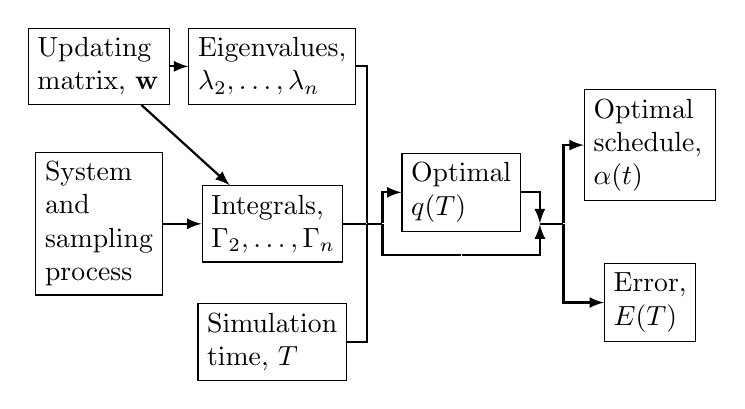
\begin{tikzpicture}
  \node[draw, text width={width("Updating ")}]
    (w) at (0, 3) {Updating \\matrix, $\mathbf w$};

  \node[draw, text width={width("sampling")}]
    (sys) at (0, 1) {System\\and\\sampling\\process};

  \node[draw, text width={width("Eigenvalues,")}]
    (lambda) at (2.2, 3) {Eigenvalues,\\$\lambda_2, \dots, \lambda_n$};

  \node[draw, text width={width("Integrals, ")}]
    (gamma) at (2.2, 1) {Integrals, \\$\Gamma_2, \dots, \Gamma_n$};

  \node[draw, text width={width("Simulation")}]
    (T) at (2.2, -0.5) {Simulation\\time, $T$};

  \node[draw, text width={width("Optimal")}]
    (qT) at (4.6, 1.4) {Optimal\\ $q(T)$};

  \node[draw, text width={width("Schedule,")}]
    (alpha) at (7, 2) {Optimal schedule,\\ $\alpha(t)$};

    \node[draw, text width={width("Error,")}]
    (err) at (7, 0) {Error, $\Err(T)$};

  \node[inner sep=0, minimum size=0] (M1) at (3.4, 1) {};

  \node[inner sep=0, minimum size=0] (N1) at (5.9, 1) {};

  \node[inner sep=0, minimum size=0] (R1) at (3.6, 1) {};
  \node[inner sep=0, minimum size=0] (R2) at (4.6, 0.6) {};
  \node[inner sep=0, minimum size=0] (R3) at (5.6, 1) {};

  \draw[->, >=latex, thick]
    (w) edge (lambda)
    (w) edge (gamma)
    (sys) edge (gamma);

  \draw[->, >=latex, thick]
    (lambda) -| (M1)
    (gamma)  -- (M1)
    (T)      -| (M1)
    (M1)     -- (R1)
    (R1)     |- (qT);

  \draw[->, >=latex, thick]
    (qT)     -| (R3);

  \draw[->, >=latex, thick]
    (R3) -- (N1) |- (alpha);

  \draw[->, >=latex, thick]
    (N1) |- (err);

  \draw[->, >=latex, thick]
    %(M1) edge[bend left=70] (N1);
    (R1) |- (R2) -| (R3);
\end{tikzpicture}
\end{singlespace}
\caption{
  \label{fig:vardep}
  Dependence of variables in computing
  the optimal schedule and the error.
}
\end{figure}




\begin{enumerate}

\item
From the updating matrix, $\mathbf w$,
compute the eigenvalues, $\lambda_k$'s.

\item
Run a preliminary adaptive FDS simulation
%using the updating scheme
with a constant updating magnitude, $a_0$.

\item
Compute $\Gamma_k$'s from Eq. \eqref{eq:varY}.

\item
Compute the optimal $q(T)$ by solving Eq. \eqref{eq:opt_qT}.

\item
Compute the optimal schedule by
numerically integrating Eq. \eqref{eq:q_opt}.

\item
  Compute the error $\Err(T)$ from
Eqs. \eqref{eq:error_split},
  \eqref{eq:error_res1},
  and
  \eqref{eq:error_asym2}.

\end{enumerate}





\subsection{\label{sec:more_wband}
Homogeneous updating schemes
}


Here, we present some detailed derivations
on the homogeneous updating schemes.
%
By the translational invariance,
homogeneous updating schemes
satisfy detailed balance,
Eq. \eqref{eq:w_detailedbalance},
for the flat distribution, $\rho_i = 1/n$,
i.e. the updating matrix, $\mathbf w$,
is symmetric.
%
The updating matrices
share the same set of eigenvectors
(which here are sines and cosines of different frequencies),
and thus are completely determined
by the eigenvalues.
%
Further, the multiplication of $\mathbf w$
can be reduced to a convolution with the window function,
or the updating kernel.
%
Thus,
there is a one-to-one correspondence between
the eigenvalues of $\mathbf w$
and the updating kernel.




\subsection{\label{sec:stabilize_wband}
Stabilization}



%A practical problem of using homogeneous updating scheme
%is the following.
%
A homogeneous updating scheme
specified by an arbitrary kernel
is not necessarily stable,
i.e. some eigenvalues can be negative.
%
%
%\note{
  %For example,
  %the triple-bin updating scheme
  %is unstable if Eq. \eqref{eq:nn_stable} is violated.
  %
%}%
Even
the Gaussian updating scheme, which is stable in the continuous limit,
can be unstable
when the updating kernel is truncated during discretization.
%
Here we show how to minimally modify
the updating kernel
to stabilize it.
%
\note{The relative code is \texttt{trimwindow()} in \texttt{invt.h}.
}


Given an updating kernel,
we can compute the eigenvalues from
Eq. \eqref{eq:wband_eigenvalue}.
%
By replacing negative eigenvalues with zeros and
using the inversion formula,
Eq. \eqref{eq:mu_from_lambda_pbc}
or \eqref{eq:mu_from_lambda_refl},
we get a new updating kernel,
which is stable by construction.
%
However, the new kernel is widened
as $\mu_l$ may be nonzero for $l > b$.
%
If we truncate the new kernel at $\mu_b$,
the stability problem remains,
although the negative eigenvalues
tend to be smaller in magnitude.
%
Thus, to stabilize the updating kernel
without increasing the width,
we need to iterate the above process many times,
resulting the following algorithm.


%
\begin{enumerate}
  \item
    Given an updating kernel, $\mu_0, \dots, \mu_b$,
    compute the eigenvalues,
    $\lambda_1, \dots, \lambda_n$,
    from Eq. \eqref{eq:wband_eigenvalue}.
  \item
    If all eigenvalues are nonnegative within the numerical error,
    we are done. % and exit the loop.
  \item
    Otherwise, replace negative eigenvalues by zeros,
    and compute the new kernel,
    $\mu_0, \dots, \mu_b$, from
    Eq. \eqref{eq:mu_from_lambda_pbc}
    or
    \eqref{eq:mu_from_lambda_refl}
    with $\mu_l = 0$ for $l > b$.
    Go to step 1.
\end{enumerate}


\section{\label{sec:upperbound}
Asymptotic error for an updating scheme
with a set of well-separated eigenvalues}


We will derive here an upper bound of the asymptotic error
that can be associated to updating schemes
with a set of well-separated eigenvalues,
in parallel to the lower bound reached by
the single-bin scheme with a set of identical eigenvalues
(cf. Sec. \ref{sec:optWL}).


Starting from the definition Eq. \eqref{eq:mass_func}, we have
$$
  M(Q)
  \le
  \sum_{k = 2}^n
  \sqrt{ \Gamma_k } \, \lambda_k \, e^{ -\lambda_k \, Q }
  .
$$
Thus,
it follows from Eq. \eqref{eq:mint} that, as $q(T) \to \infty$,
%
\begin{equation}
  C
  =
  \int_0^\infty
  M(q') \, dq'
  \le
  \sum_{k = 2}^n \sqrt{ \Gamma_k }
  ,
  \label{eq:mint_ubound}
\end{equation}
%
and the asymptotic error from Eq. \eqref{eq:error_asym2}
is bounded as
\begin{equation}
  \Err_A(T)
  =
  \frac{ C^2 } { T }
  \le
  \frac 1 T
  \left(
    \sum_{k=2}^n \sqrt{ \Gamma_k }
  \right)^2
  .
  \label{eq:error_asym_ubound}
\end{equation}
%
It is readily seen that this bound is always
greater than the lower bound given by Eq. \eqref{eq:error_asym_singlebin},
%
$$
\frac{T}{(T+t_0)^2} \, \sum_{k=2}^n \Gamma_k
\le
\frac{1}{T} \sum_{k=2}^n \Gamma_k
\le
\frac{1}{T} \left( \sum_{k=2}^n \sqrt{ \Gamma_k } \right)^2
.
$$



Next, we will show that this bound represents
updating schemes with a set of very different eigenvalues.
%
%First, observe that the summand of Eq. \eqref{eq:mass_func},
%$\Gamma_k \, \left( \lambda_k e^{-\lambda_k \, Q} \right)^2$
%is a function that peaks at $\lambda_k = 1/Q$,
%so that the sum is dominated by the term at $k = k(Q)$ with
%%
%\begin{equation}
%  \lambda_{k(Q)}
%  \approx
%  \frac 1 Q
%  .
%  \label{eq:kQ_def}
%\end{equation}
%
%Thus,
First, we have for any mode $k^*$ $(k^* \ge 2)$,
%
\begin{align}
  M(Q)
  &
  \ge
  %\approx
  \sqrt{ \Gamma_{ k^* } } \,
  \lambda_{ k^* } \,
  e^{ -\lambda_{ k^* } \, Q }
  ,
\label{eq:MQ_lbound1}
\end{align}
%
which would approach an equality if the $k^*$ mode
dominates the mass function, $M(Q)$,
as defined in Eq. \eqref{eq:mass_func}.
%
Then, for the $k$th component of the asymptotic error,
we have from Eq. \eqref{eq:error_asym_Lagrangian}
%
\begin{align}
  \left\langle
  y_k^2(T)
  \right\rangle_A
  &=
  \int_0^T
  \Gamma_k \, \lambda_k^2 \, e^{2 \, \lambda_k \, [q(t) - q(T)] }
  \, {\dot q}^2(t) \, dt
  \notag
  \\
  &=
  \frac{ C } { T }
  \, \Gamma_k \, \lambda_k^2
  \int_0^{q(T)}
  \frac{ e^{-2 \, \lambda_k \, Q } } { M(Q) }
  \,  \, dQ
  \notag
  \\
  &\le
  \frac C T \,
  \frac{ \Gamma_k \, \lambda_k^2 } { \sqrt{ \Gamma_{k^*} } \, \lambda_{k^*} }
  \int_0^{q(T)}
    e^{-(2 \, \lambda_k - \lambda_{k^*} ) \, Q}
    \, dQ
  \notag
  \\
  &\le
  \frac C T \,
  \cdot
  \frac{ \Gamma_k }
  { \sqrt{ \Gamma_{k^*} } }
  \cdot
  \frac{ \lambda_k^2 }
  { \lambda_{k^*} \, (2 \, \lambda_k -\lambda_{k^*}) }
  ,
  \label{eq:y2_ubound_k}
\end{align}
%
where we have
used Eqs. \eqref{eq:Lagrangian_const} and \eqref{eq:MQ_lbound1}
on the second and third lines, respectively,
and extended the upper limit to infinity on the last line.
%
For a set of well-separated eigenvalues,
$\lambda_k$ depends on the mode index, $k$,
much more critically than $\Gamma_k$.
%
Thus, the tightest upper bound
can be approximately obtained from minimizing the last factor
on the right-hand side of Eq. \eqref{eq:y2_ubound_k},
and the minimal is reached at $k^* = k$,
when $\lambda_{k^*} = \lambda_k$.
%
So
%
\begin{equation}
  \left\langle
  y_k^2(T)
  \right\rangle_A
  \le
  %\approx
  \frac C T
  \sqrt{ \Gamma_k }
  .
  \label{eq:y2_ubound}
\end{equation}
%
By summing over $k$
and using Eq. \eqref{eq:mint_ubound},
we recover Eq. \eqref{eq:error_asym_ubound}.

This result shows that with a set of well-separated eigenvalues,
the asymptotic error profile would be
independent of $\lambda_k$'s and
be flatter than the initial one from
Eq. \eqref{eq:y2_eql}
(cf. Fig. \ref{fig:xerr}
for a Gaussian example).
%
Note, however, that to approach this upper bound
the simulation has to be long enough
such that the upper limit of the integral
can be extended from $q(T)$ to infinity
in the last step of Eq. \eqref{eq:y2_ubound_k}.
%
As a result,
the flatter profile from Eq. \eqref{eq:y2_ubound}
would stop at mode $k$,
at which $\lambda_k \approx 1/q(T)$.
%In other words,
%the above asymptotic limit fails around
%$Q^* \approx q(T)$, or equivalently
%around mode $k^* = k\bigl( q(T) \bigr)$,
%where $\lambda_{ k^* } \approx 1/q(T)$.
%%
%\note{This case also exemplifies
%  the sensitivity to the simulation length.
%  %
%  In this limit,
%  $M(Q) \propto 1/Q$ by Eq. \eqref{eq:MQ_lbound},
%  and $C \propto \ln\bigl[ q(T) / q_0 \bigr]$
%  for some $q_0$,
%  and we expect that with fixed $a_0$,
%  $q(T)$ to increase almost linearly with $T$
%  by Eq. \eqref{eq:opt_qT}.
%  %
%  So the normalized asymptotic error,
%  $E_A \cdot T \propto \bigl( \ln[ q(T)/q_0 ] \bigr)^2 \sim (\ln T)^2$,
%  is sensitive to the simulation length,
%  and worse than the ideal case of a constant.
%}




\section{\label{sec:invt_schedule}
Modified inverse-time schedules}



Here we compute the error of the schedule given by
the modified inverse-time formula,
Eq. \eqref{eq:alpha_invtlambda}.
%As an alternative to the
%optimal schedule from Eq. \eqref{eq:q_opt},
%here we consider the modified
%inverse-time formula, Eq. \eqref{eq:alpha_invtlambda},
%with a free parameter $\lambda$.
%
%whose error can be computed explicitly.



\subsection{\label{sec:invt_error}
General results on error
}



Using Eq. \eqref{eq:alpha_invtlambda}
in Eq. \eqref{eq:error_asym1} yields
the asymptotic error
%
\begin{align}
  \Err_A(T)
  &=
  \frac{    1    }
       { T + t_0 }
  \sum_{k = 2}^n
    \frac{ \Gamma_k \, \nu_k^2 }
         {    2 \, \nu_k - 1   }
  \left[
    1 - \left(
          \frac {     t_0 }
                { T + t_0 }
        \right)^{ 2 \, \nu_k - 1 }
  \right]
  ,
\label{eq:error_asym_invt}
\end{align}
%
where $\nu_k \equiv \lambda_k / \lambda$.
%
From Eq. \eqref{eq:error_res1},
we get the residual error
%
\begin{equation}
  \Err_R(T)
  =
  \frac { a_0 } { 2 }
  \sum_{k = 2}^n
  \Gamma_k \, \lambda_k \,
  \left(
      \frac{   t_0   }
           { T + t_0 }
  \right)^{ 2 \, \nu_k }
  .
\notag
%\label{eq:error_res_invt}
\end{equation}
%
The total error is the sum of the two.
%with
%$
%  q(T)
%  =
%  ( 1 / \lambda )
%  \ln\left(
%    1 + T / t_0
%  \right)
%$
%%
%from integrating Eq. \eqref{eq:alpha_invtlambda}.
%
%We assume that
%the system was initially equilibrated
%at a constant $a_0$,
%such that the values of
%$\left\langle y_k^2(0) \right\rangle$
%can be computed from Eq. \eqref{eq:y2_eql},
%as well as Eq. \eqref{eq:t0_sinc}.
%
%The total error is
%%
%\begin{align}
%\Err
%&=
%\Err_R + \Err_A
%\notag
%\\
%&=
%\sum_{ k = 2 }^n
%  \frac
%  {
%    \Gamma_k \, \nu_k \,
%    \left[
%      \nu_k
%      +
%      (\nu_k - 1)
%      \left(
%        \frac{ t_0 } { T + t_0 }
%      \right)^{ 2 \, \nu_k - 1 }
%    \right]
%  }
%  {
%    (T + t_0) \, (2 \, \nu_k - 1)
%  }
%  .
%%\notag
%\label{eq:error_invt}
%\end{align}




\subsection{\label{sec:invt_singlebin}
  Single-bin updating scheme
}



For the single-bin scheme, we have
$\lambda_2 = \cdots = \lambda_n = 1$,
and
$\Gamma_k$'s affect the error
only via the sum, $\sum_{k = 2}^n \Gamma_k$,
as a multiplicative constant.

In the asymptotic limit,
we can focus on the asymptotic error
and drop the second term in the square brackets
of Eq. \eqref{eq:error_asym_invt}
by assuming $\lambda < 2$.
%
Then,
$$
  \Err_A(T)
  =
  \frac { 1 } { T + t_0 }
  \frac {             1            }
        { \lambda \, (2 - \lambda) }
  \sum_{ k = 2 }^n \Gamma_k
  ,
$$
is minimal at $\lambda = 1$.
%
\note{A higher-order correction:
  $
  \lambda = 1 -
  \left[
    1 - \frac 1 2 a_0 \, (T+t_0)
  \right] r \, \log r
  ,
  $
  where $r = t_0 / (T + t_0)$.
}




\subsection{\label{sec:invt_nn}
Triple-bin updating scheme}




For the triple-bin updating scheme,
%introduced in Sec. \ref{sec:nnscheme},
we can find an analytical expression
of the optimal value of $\lambda$
in the large-$n$ and asymptotic limit.
%
In this case,
if $2 \, \nu_k > 1$ for every $k$,
the asymptotic error is implicitly given by the integral
%$\sum_i \to \frac{2 \, n}{\pi} \int_0^{\pi/2} dp$, and
%
\begin{align}
  \Err_A(T)
  =
  \frac{ 2 \, n  }
       { \pi \, T }
  \int_0^{\pi/2}
    \frac{ \Gamma(p) \, \left(1 - 4 \, \mu_1 \, \sin^2 p \right)^2    }
         {   \lambda \, \left(2 - 8 \, \mu_1 \, \sin^2 p - \lambda \right) }
  \, dp
  .
\notag
%\label{eq:error_nn_asym_int}
\end{align}



For perfect sampling, if $\mathbf p = \pmb \rho$,
we have
$\Gamma(p) = 1$ from Eq. \eqref{eq:Gamma_perfect},
and
$$
\begin{aligned}
  \Err_A(T)
  &=
  \frac{n}{4 \, T}
  \left(
    \frac{2 - 4 \, \mu_1 + \lambda}{ \lambda }
    +
    \frac{ \lambda }
    { \sqrt{ (2 - \lambda) (2 - 8 \, \mu_1 - \lambda) } }
  \right)
.
\end{aligned}
$$
%
Minimizing the function yields
%
\begin{equation}
  \lambda
  =
  \frac{ 1 - 4 \, \mu_1 }
       { 1 - 2 \, \mu_1 }
  ,
%\notag
\label{eq:lambda_nn_perfect}
\end{equation}
%
which shows that the original inverse-time formula,
Eq. \eqref{eq:alpha_invt1},
is not optimal in this case.
%
The asymptotic error is given by
%
\begin{equation}
  \Err_A(T)
  =
  \frac{n}{T}
  \left(
    1+ \frac{2 \, \mu_1^2}{1-4 \, \mu_1}
  \right)
  ,
\notag
%\label{eq:error_nn_perfect}
\end{equation}
%
%From Eq. \eqref{eq:error_nn}, it is clear that
which
is minimal at $\mu_1 = 0$, the single-bin case.
%increases with the magnitude of $\mu_1$
%no matter its sign,
%and the minimal value, obtained at $\mu_1 = 0$,
%corresponds to the single-bin scheme.
%
Note that the value given by
Eq. \eqref{eq:lambda_nn_perfect}
was less than the observed optimal value
from Fig. \ref{fig:errinvt},
and the latter would decrease
with the simulation length.
%




For the one-step sampling process,
we find from Eq. \eqref{eq:Gamma_onestep}
that $\Gamma(p) = \cot^2 p$
peaks around $p \approx 0$,
%
Then
$$
  \Err_A(T)
  \propto
  \frac{   2 \, n }
       { \pi \, T }
  \frac{             1             }
       {  \lambda \, (2 - \lambda) }
  .
$$
%
The optimal $\lambda$ is, therefore,
$\lambda \approx 1$.
%

\note{
However, the above result %Eq. \eqref{eq:lambda_nn_onestep}
is only good
for sufficiently short simulations,
since we have taken the limit of $n \to \infty$
for a fixed $T$.
%
For very long simulations,
the optimal $\lambda$
will ultimately drift to
the smallest eigenvalue,
$\min \lambda_k = 1 - 4 \, \mu_1$.
}


\note{The table of symbols is listed in Table \ref{tab:symbols}.
  \begin{table*}
  \footnotesize
  \centering
  \rowcolors{1}{white}{LightGray}
  \setlength{\tabcolsep}{4pt} % column separation
  %
  \caption{\label{tab:symbols}Table of symbols.}
  \begin{tabular}{l | p{12cm} }
    Symbol          &   Description \\
    \hline
    $\mathbf{A}$    &   Transition matrix. \\
    $\alpha$        &   Updating magnitude. \\
    $b$             &   Cutoff of the kernel of homogeneous updating schemes. \\
    $C$             &   $C \equiv \int_0^{ q(T) } M(Q) \, dQ$.  \\
    $\delta$        &   Dirac's or discrete $\delta$-function. \\
    $c$             &   Constant. \\
    $\Err, \Err_R, \Err_A$          &   Error, residual error, asymptotic error. \\
    $\ln f$         &   Updating factor in the WL algorithm.  \\
    $\phi_{ki}$     &   Eigenvectors of the updating matrix. \\
    $g$             &   Degeneracy factor, $2$ for a periodic variable, or for $1$ a non-periodic one. \\
    $\Gamma_k$      &   Integral of the autocorrelation function of mode $k$. \\
    $h_i(t)$        &   Instantaneous histogram.  \\
    $H_i$           &   Average normalized histogram.  \\
    $i, j$          &   Bin indices. \\
    $\lambda_k$     &   The $k$th eigenvalue of the updating matrix. \\
    $k, l$          &   Mode indices. \\
    $K$             &   Cutoff wave number of bandpass updating schemes.  \\
    $\kappa_k(t)$   &   Autocorrelation function of mode $k$. \\
    $M(Q)$          &   Mass function, Eq. \eqref{eq:mass_func}.   \\
    $m(Q)$          &   Mass distribution,
                        $m(Q) \equiv M(Q)/\int_0^{ q(T) } M(Q') \, dQ'$.  \\
    $\mu_i$         &   Updating kernel of a homogeneous updating scheme. \\
    $n$             &   Number of bins. \\
    $\nu_k$         &   $\nu_k \equiv \lambda_k / \lambda$. \\
    $p_i$           &   Distribution. \\
    $\pi_i$         &   (Instantaneous) distribution, Eq. \eqref{eq:pi_p_V}. \\
    $q(t)$          &   $\int_0^t \alpha(t') \, dt'$.  \\
    $Q$             &   $q(T) - q(t)$.  \\
    $\theta_k(t)$   &   Noise of mode $k$, Eq. \eqref{eq:theta_def}. \\
    $\rho_i$        &   Distribution used to define the error. \\
    $s, S$          &   Stage index and the total number of stages in the Wang-Landau algorithm. \\
    $\sigma_{ij}(t)$   &   Autocorrelation function of $\zeta_i(t)$. \\
    $\sigma$        &   Width of the Gaussian updating scheme. \\
    $t, \tau$       &   Time. \\
    $T$             &   Simulation length. \\
    $u_i(q')$       &   $u_i(q') \equiv e^{\lambda \, [q - q(T)]}$. \\
    $V_i(t)$        &   Original bias potential. \\
    $v_i(t)$        &   Shifted bias potential. \\
    $\mathbf w$     &   Updating matrix. \\
    $x_i(t)$        &   Average-deducted bias potential, Eq. \eqref{eq:x_def}. \\
    $\xi_i(t)$      &   The noise, Eq. \eqref{eq:xi_def}. \\
    $y_k(t)$        &   Mode of the shifted bias potential, Eq. \eqref{eq:y_def}. \\
    $Y_k$           &   Mode of the original bias potential, Eq. \eqref{eq:Y_def}. \\
    $z$             &   Reaction coordinate. \\
    $\zeta_i(t)$    &   The noise part of the instantaneous histogram, $h_i(t)$.
  \end{tabular}
  \end{table*}
}

\bibliography{simul}
\end{document}
